%% LyX 2.1.4 created this file.  For more info, see http://www.lyx.org/.
%% Do not edit unless you really know what you are doing.
\documentclass[oneside,english]{amsart}
\usepackage{lmodern}
\renewcommand{\sfdefault}{lmss}
\renewcommand{\ttdefault}{lmtt}
\usepackage[T1]{fontenc}
\usepackage[latin9]{inputenc}
\usepackage[letterpaper]{geometry}
\geometry{verbose}
\setcounter{secnumdepth}{2}
\setcounter{tocdepth}{2}
\setlength{\parskip}{\medskipamount}
\setlength{\parindent}{0pt}
\usepackage{color}
\usepackage{float}
\usepackage{amstext}
\usepackage{amsthm}
\usepackage{amssymb}
\usepackage{graphicx}
\usepackage{wasysym}

\makeatletter

%%%%%%%%%%%%%%%%%%%%%%%%%%%%%% LyX specific LaTeX commands.
\floatstyle{ruled}
\newfloat{algorithm}{tbp}{loa}
\providecommand{\algorithmname}{Algorithm}
\floatname{algorithm}{\protect\algorithmname}

%%%%%%%%%%%%%%%%%%%%%%%%%%%%%% Textclass specific LaTeX commands.
\numberwithin{equation}{section}
\numberwithin{figure}{section}
\theoremstyle{plain}
\newtheorem{thm}{\protect\theoremname}

%%%%%%%%%%%%%%%%%%%%%%%%%%%%%% User specified LaTeX commands.
\usepackage{tikz}
\usepackage{graphicx}
\usetikzlibrary{shapes.multipart}
\usetikzlibrary{decorations.pathreplacing}
\setcounter{tocdepth}{4}
\setcounter{secnumdepth}{4}

\makeatother

\usepackage{babel}
\usepackage{listings}
\providecommand{\theoremname}{Theorem}
\renewcommand{\lstlistingname}{Listing}

\begin{document}
\tableofcontents{}


\part{Foundations}


\subsection*{Insertion Sort}

Maintains the invariant that $A\left[1:j-1\right]$ is sorted by shifting
elements right until $A\left[j\right]$ is in the correct position.
Insertion sort is \emph{stable}, i.e. two keys already in sorted order
remain in the same order at the end. Running time is $O\left(n^{2}\right)$.


\subsection*{Selection Sort}

Maintains the same invariant as Insertion Sort but does so by going
forward and \emph{selecting} the smallest element each time and placing
it at the head. Running time is $O\left(n^{2}\right)$.


\subsection*{Bubble Sort}

``Bubble up'' pair by pair. Stop when no more ``bubblings'' are
possible. Running time is $O\left(n^{2}\right)$.


\subsection*{Merge Sort}

Divide and conquer approach. Divide the array in half, recurse, combine
results by merging, i.e. taking the smallest entry from each piece
in turn. Base case is just an array with one element. Running time
is $O\left(n\lg n\right)$.


\subsection*{Binary search}

If an array is already sorted then you can find an element in it faster
than $O\left(n\right)$ time; you can find it in $O\left(\lg n\right)$
time. Search in either the left side of the middle entry or the right
side.


\subsection*{Horner's Rule}

Given $A=\left[a_{1},\dots,a_{n}\right]$ the coefficients of a polynomial
and a value $x$ a faster way to calculate $p\left(x\right)$ is 
\[
p\left(x\right)=\sum_{k=1}^{n}a_{k}x^{k}=a_{1}+x\left(a_{2}+x\left(a_{3}+\cdots+x\left(a_{n-1}+xa_{n}\right)\right)\right)
\]


i.e. $p_{0}=0,\ p_{1}=a_{n}+xp_{0},\ p_{2}=a_{n-1}+xp_{1},\ \dots$
.


\subsection*{Unweighted simple reservoir sampling}

Sample $k$ items from $n$ items $A=\left[a_{1},\dots,a_{n}\right]$
fairly, i.e. uniform random, \textbf{without replacement}, draws.
Put the first $k$ items into a \emph{reservoir $R$} then for item
$i>k$ draw $j\in\left\{ 1,\dots,i\right\} $ inclusive. If $i\leq k$
the replace $i$th item. Running time is $\Theta\left(n\right)$.


\subsection*{Unweighted complicated reservoir sampling}

Use a Max-Queue: generate a uniform random number for first $k$ items
and insert, then thereafter generate uniform random and insert if
less than max (also pop max). Running time takes $O\left(n\lg k\right)$
because of potentially $n$ \texttt{Extract-Max }operations on a $k$
length priority queue\texttt{.}


\subsection*{Weighted reservoir sampling}

Use the same technique as for unweighted complicated but let the priority
be
\[
u=\left(\texttt{random}\left(\right)\right)^{1/w}
\]
where $w$ is the weight of the element. Same running time.


\subsection*{Online Maximum}

Fill a reservoir with $n/e$ candidates and pick the maximum from
the reservoir. Then pick the next maximum (if one exists) that's higher;
this will be the single selection. This can be further simplified
by realizing you don't need to keep the entire reservoir and you can
return after the first forthcoming maximum (if one exists). Probability
of actually picking the max is $1/e$.


\subsection*{Stable Matching}

Gale-Shapley: first each man proposes to the woman he prefers best
and each woman accepts provisionally, i.e. accepts a proposal but
trades up if a more desirable man proposes. Do this for $n$ rounds
(or until there are no more unengaged men). Running time is $O\left(n^{2}\right)$.


\part{Sorting and Order Statistics}


\subsection*{Heaps}

The invariant for a Max heap is $A\left[i\right]\leq A\left[\left\lfloor i/2\right\rfloor \right]$.
Furthermore each entry has ``children'': $A\left[2i\right]$ is
the left child and $A\left[2i+1\right]$ is the right child of element
$A\left[i\right]$. 


\subsubsection{Max Heapify}

To re-establish the heap property switch the violator with its largest
child and then recurse. Running time is $O\left(\lg n\right)$.


\subsubsection{Build Max Heap}

To build a heap from an array notice that the deepest children/leaves
are already legal heaps so there's no need to \texttt{Max-Heapify
}them, and the children start at $\left\lfloor \text{len}\left(A\right)/2\right\rfloor $.
Running time is $O\left(n\right)$. 


\subsubsection{Extract Min}

$A\left[1\right]$ is the maximum element in the heap. Remove $A\left[1\right]$
and replace with the last element in the heap and then re-establish
the invariant using Max-Heapify from there. Running time is $O\left(\lg n\right)$.


\subsubsection{Heap sort}

You can use \texttt{Extract-Min} in the obvious way to sort an array.
Running time is $O\left(n\lg n\right)$. 


\subsubsection{Heap increase key}

This just involves re-establish the Max heap invariant by ``percolating''
the entry up the array. Running time is $O\left(\lg n\right)$.


\subsubsection{Heap insert}

Using \texttt{Heap-Increase-Key} we can insert into the heap by inserting
an $-\infty$ priority element at the end of the heap and then increasing
the key to what we want. Running time is $O\left(\lg n\right)$.


\subsection*{Quicksort}

Quicksort is experimentally the most efficient sorting algorithm.
The randomized version runs in $O\left(n\lg n\right)$ but is typically
faster. Pick a random pivot, swap it to the end, partition the rest
of the array (not including the end) on whether elements are $\leq$
or $>$, recurse, and finally insert the pivot in between the two
sorted partitions. 


\subsection*{Counting Sort}

Given keys in the range $1,\dots,k$ count the number of keys less
than or equal to each key $a_{i}$ and then places $a_{i}$ in that
position (but do it in reverse in order for the sort to be stable).
Note that if there are duplicates you need to subtract from cumulates
when some $a_{i}$ is placed. Running time is $O\left(n+k\right)$.

\begin{algorithm}[H]
\noindent \begin{raggedright}
\texttt{Counting-Sort}$\left(A\right)$
\par\end{raggedright}

\begin{lstlisting}[basicstyle={\ttfamily},language=Python,mathescape=true,numbers=left,showstringspaces=false,tabsize=3]
$ k = \max\left(A\right)$
$ C = \left(k+1\right)*\left[0\right]$
# count how many of values from $1$ to $k$ there is
for $i = 1:\text{len}\left(A\right)$:
	$C\left[A\left[i\right]\right] =C\left[A\left[i\right]\right] + 1$
# count how entries in $A$ less or equal to $i$
for $i = 1: k$:
	$C\left[i\right] = C\left[A\left[i\right]\right] + 1$
# now place the items in the correct places
$ B = \left(k+1\right)*\left[None\right]$
# go in reverse direction in order for sort to be stable
for $i = \text{len}\left(A\right):1$:
	# $a_i$ has $C\left[a_i\right]$ elements to its left in $B$
	$B\left[C\left[A\left[i\right]\right]\right] = A\left[i\right]$
	# if there are multiples of $a_i$ then the next 
	# should be left of in order for stable
	$C\left[A\left[i\right]\right] = C\left[A\left[i\right]\right] -1 $
\end{lstlisting}
\end{algorithm}



\subsection*{Radix Sort}

Sort stably least significant to most significant digit. For $n$
numbers in base $d$ where each digit ranges from $1$ to $k$ the
running time is $\Theta\left(d\left(n+k\right)\right)$ if the stable
sort runs in $\Theta\left(n+k\right)$.


\subsection*{Bucket Sort}

Bucket sort depends on values being uniformly distributed $\left[0,1\right]$.
It buckets all the entries into $\left\lfloor n\cdot A\left[i\right]\right\rfloor $
and then subsorts. Expected run time is $\Theta\left(n\right)$.


\subsection*{Order statistics}


\subsubsection{Quickselect}

Any sorting algorithm can be used to compute $k$th order statistics:
simply sort and return the $k$th element. But using the ideas of
\texttt{Quicksort} you can get down to expected time $O\left(n\right)$:
only recurse to one side.


\subsubsection{Quickerselect}

Using \emph{median-of-medians} (divide into groups of 5, sort to find
median of group, then recurse to median of medians) in order to guarantee
good splits. Then recurse either left or right (instead of both partitions).
Running time is $O\left(n\right)$ deterministically, instead of just
expected.


\part{Data Structures}


\subsection*{Hash Tables}

Hash tables are $m$ length arrays keyed on strings instead of numbers.


\subsubsection{Hash function}

A good hash function according to Knuth is 
\[
h\left(k\right)=\left\lfloor m\left(kA\mod1\right)\right\rfloor 
\]
where $A\approx\left(\sqrt{5}-1\right)/2$ and $kA\mod1$ means the
fractional part of $kA$, i.e. $kA-\left\lfloor kA\right\rfloor $.


\subsubsection{Hashing with chaining }

Hashing with chaining is basically Bucket Sort, except with the $\left\lfloor \right\rfloor $
replaced by a Hash function and retrieval. If $n$ is the total number
of items in the hash table and $m$ is the length of the hash table
then on average (give uniform hashing) each list has $\alpha=n/m$
items. Therefore insertion is $\Theta\left(1\right)$, and retrieval/deletion
is $\Theta\left(1+\alpha\right)$.


\subsubsection{Hashing with open addressing}

In hashing with open addressing the buckets are ``linearized'',
i.e. just laid out in the table itself: inserts and searches hash
and then traverse forward in the table until they find a spot. Deletion
is harder so if deletion is necessary then hashing with chaining should
be used. Insertion costs at most $1/\left(1-\alpha\right)$ and for
$\alpha<1$ retrieval costs 
\[
\frac{1}{\alpha}\ln\left(\frac{1}{1-\alpha}\right)
\]
Integral to these bounds is that $\alpha$ the load factor stay small.
In order for the amortized analysis to workout the hash table should
be doubled in size (and entries copied) when the table becomes full
but halve it only when the load goes down to below $1/4$\@.


\subsection*{Binary Search Tree}

A binary tree is a graph where each vertex has at most two children.
A binary search tree is a tree with the further constraint that the
key of a parent is greater or equal to any of the keys in its left
subtree and less than or equal to any of the keys in its right subtree.


\subsubsection{Inserting into a binary search tree}

Start at the root, if the root value is equal to the key you're inserting
then go left, otherwise go right. Once you hit a \texttt{None }create
a new vertex. Running time is $O\left(\lg n\right)$ if the tree is
balanced.


\subsubsection{Searching a binary search tree}

Start at the root, if the root value is equal to the key you're searching
for then you're done, otherwise if the key is less than the value
go left, otherwise go right. Running time is $O\left(\lg n\right)$
if the tree is balanced.


\subsubsection{Binary search tree min/max}

The minimum of a binary tree is the left-est most vertex. Running
time is $O\left(\lg n\right)$ if the tree is balanced.

The maximum of a binary tree is the right-est most vertex. Running
time is $O\left(\lg n\right)$ if the tree is balanced.


\subsubsection{Binary search tree predecessor/successor}

The predecessor of a vertex the maximum of a vertex's left subtree.
Running time is $O\left(\lg n\right)$ if the tree is balanced.

The successor of a vertex the minimum of a vertex's right subtree.
Running time is $O\left(\lg n\right)$ if the tree is balanced.


\subsubsection{Deleting from a binary search tree}

Replace with predecessor or successor (be careful about patching up
all the pointers and the original site of the replacement). Running
time is $O\left(\lg n\right)$ if the tree is balanced.


\subsubsection{Pre-order/In-order/Post-order traversal}

Either do the thing before/in between/after recursing into left-child/left-child
and right-child/right-child.


\subsection*{Treap}

A treap combines the invariants of a binary tree \emph{and} and a
heap. There are two sets of attributes: priorities and keys. The priorities
obey the heap property (children have smaller priority than their
parents) and the keys obey the binary search property. In order to
get a balanced binary tree, which is the value of treaps, we randomly
generate a priority key.


\subsubsection{Treap search}

Just like for binary search tree and hence omitted.


\subsubsection{Treap insert}

This is easier of the two operations. First we need two auxiliary
functions \texttt{Left-Rotate} and \texttt{Right-Rotate}. The easiest
way to remember these is pictures

\begin{figure}[H]
\noindent \centering{}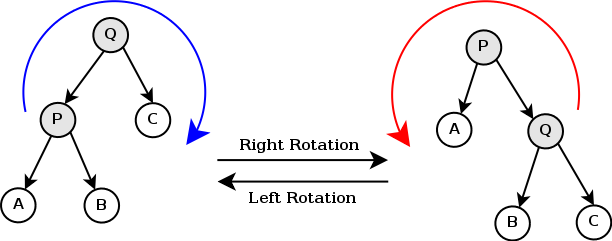
\includegraphics[scale=0.5]{Tree_rotation}
\end{figure}


To insert into a treap, generate a random priority, and insert the
key as if it were a binary search tree (i.e. at the bottom), then
rotate up until the heap property is restored. Running time is $O\left(\lg n\right)$.


\subsubsection{Treap delete}

To delete a vertex rotate it down until it's a leaf node and then
delete the leaf node. Rotate down according to which of the vertex's
children have a higher priority: if the left child has a higher priority
than the right then rotate right (i.e. replace the vertex with its
largest child, just like for Heaps), otherwise rotate left.


\subsection*{Cartesian Tree}

Given a sequence of \textbf{distinct} numbers (or any totally ordered
objects), there exists a binary min-heap whose inorder traversal is
that sequence. This is known as the Cartesian tree for that sequence.
How to construct a Cartesian tree for an arbitrary sequence $A=\left[a_{1},\dots,a_{n}\right]$?
Process the sequence values in left-to-right order, maintaining the
Cartesian tree of the nodes processed so far, in a structure that
allows both upwards and downwards traversal of the tree. To process
each new value $x$, start at the node representing the value prior
to $x$ in the sequence and follow the path from this node to the
root of the tree until finding a value $y$ smaller than $x$. This
node $y$ is the parent of $x$, and the previous right child of $y$
becomes the new left child of $x$. Running time is $O\left(n\right)$.


\subsection*{Skip Lists}

Skip lists are another easy to have $O\left(\lg n\right)$ expected
time Insert, Search, Delete, and even find by Rank. 

The basic idea is to use a \textbf{sorted} linked list but to skip
ahead (duh) as many entries when performing some operation, e.g. when
searching skip ahead 2 entries until you've passed the entry you were
looking for. How do implement the ability to skip ahead by 2? Simple:
have links not only between consecutive nodes but also every two nodes.
The obvious generalization is to also have links every 4 nodes, 8
nodes, etc. Call these nodes which have links to $k$ nodes level-$k$
nodes. 

Max level is $\log_{2}n$ where $n$ is expected size. Max level is
the height of the header.


\subsubsection{Search}

Start at the current highest level of the list at the header. Go right
while the next key is greater than the key you're looking for, then
go down one level, and go right again. Expected running time is $O\left(\lg n\right)$.


\subsubsection{Insertion}

Search for the spot for the entry (all the way from the top this time)
while keeping track of the ``staircase'' you descended down. Generate
a random height using $k=1-\log_{2}\left(\texttt{random}\left(\right)\right)$
and insert the node, patching up pointers and potentially adjusting
the new highest extant level. Expected running time is $O\left(\lg n\right)$.


\subsubsection{Deletion}

Deletion works pretty similarly to insert except that when potentially
decrementing highest extant level you should start at the current
level and decrement until the pointer from the header hits something.
Expected running time is $O\left(\lg n\right)$.


\subsection*{Interval Trees}

An interval tree is built atop your favotire balanced binary tree
data structure and stores left endpoints as key. It also keeps track
of maximum right endpoint in the subtree rooted at a vertex. It supports
interval intersection tests (very useful). Maintaining the max in
insertion and deletion is straightforward during rotations.


\subsubsection{Interval search}

Interval search works by being optimistic: $i=\left[a,b\right]$ and
$j=\left[x,y\right]$ two intervals overlap if either $a\leq x\leq b$
or $x\leq a\leq y$. Therefore at each interval we test for overlap
and whether $x\leq a\leq y$ where $y$ is the maximum right endpoint
for any interval in the left subtree. If so we go left. If in fact
$y<a$ then no interval in the left subtree could possibly intersect
so we go right. Running time is $O\left(\lg n\right)$.


\subsection*{Order Statistics Tree}

Order statistics trees are probably the simplest thing to build atop
a balanced binary search tree. The only extra extra piece of information
each vertex stores is the attribute \texttt{size }where $x\left[\texttt{'size'}\right]=x\left[\texttt{'lchild'}\right]\left[\texttt{'size'}\right]+x\left[\texttt{'rchild'}\right]\left[\texttt{'size'}\right]+1$.


\subsubsection{Select}

Finding the $i$th ordered element in the tree works just like Quickselect.
The only trick is that if you recurse into the right child then you're
looking for $i-r$ where $r$ is the size of the element where you're
currently at (i.e. rank of left child plus 1).


\subsubsection{Rank}

We can find the rank of an element by finding how many elements are
to its left. The rank of an element is at least size of its left child
plus 1, but the element might be in a right subtree of some other
element, therefore we need to count the sizes of the trees to its
left. Hence head towards the root: if vertex is right child of parent
then there are $\left(\text{rank of parent's left child}\right)+1$
elements to the vertex left, and otherwise (if vertex is left child)
then we just keep going.


\subsubsection{Maintenance}

Maintaining \texttt{size }is easy: for example in \texttt{Left-Rotate
}add lines \\
\\
13 $y\left[\texttt{'size'}\right]=x\left[\texttt{'size'}\right]$\\
14 $x\left[\texttt{'size'}\right]=x\left[\texttt{'lchild'}\right]\left[\texttt{'size'}\right]+x\left[\texttt{'rchild'}\right]\left[\texttt{'size'}\right]+1$

and similarly for \texttt{Right-Rotate.}


\subsection*{Union-Find}

A union-find data structure is a data structure suited for taking
unions and finding members (duh). The particular units of the data
structures are sets (not hash table derivatives), each with a representative.
The data structure is very thin, basically a wrapper for the primitive
data, except for a pointer to the representative of the set and two
heuristics that speed up the operations. The path compression heuristic
``compresses'' the path to representative of the set by setting
it to be equal to that representative (which it might not be after
a union). The weighted union heuristic makes it so that the smaller
of the two sets unioned is the one whose representative pointers need
to be updated.

Amortized complexity of $n$ \texttt{Make-Set}, \texttt{Find-Set,
Union,} operations where $m$ are \texttt{Make-Set} is $O\left(m\alpha\left(n\right)\right)$
where $\alpha\left(n\right)$ is the Ackermann function and $\alpha\left(n\right)\leq4$
for any realistic application. 


\subsubsection{Make set}

Just wrap the element in a dict.


\subsubsection{Find set}

Recursively look for the set of a set's representative. Also unwinds
the stack in order to reset all the representatives in the chain from
$x$ to the representative of the set, to the representative of the
set.


\subsubsection{Union}

Union by the weighting heuristic: the set with the smaller number
of elements should become the representative of the bigger set. If
the weights are equal then one of theirs rank should be incremented.


\subsection*{Euler circuit}

An Euler circuit visits each vertex in graph twice - once going past
it and once coming back across it. How do you print out an Euler circuit
of a tree? Use a modified depth first traversal: print before entering
the child traversal loop and then print again after recursing into
the children.


\subsection*{Tarjan's Least Common Ancestor}

The least common ancestor $w$ of two vertices $u,v$ in a tree is
the ancestor common to both that's of greatest depth. The algorithm
is useful for range-minimum querying. It uses the same traversal as
\texttt{Euler-Circuit} and the Union-Find data structure augmented
with a property \texttt{ancestor}. The algorithm proceeds by growing
``bottom up'' sets corresponding to subtrees whose roots are the
least common ancestors of any pair of vertices in the tree \textbf{which
have been completely traversed by the Euler circuit}. Let $P$ be
a global with the set of vertices you're interested in finding least
common ancestor of and initialize all vertices to have \texttt{color
}\textcolor{blue}{Blue} in order to represent unfinishined (i.e. not
completely traversed by the Euler circuit).

\begin{algorithm}[H]
\noindent \begin{raggedright}
\texttt{Least-Common-Ancestor}$\left(u\right)$
\par\end{raggedright}

\begin{lstlisting}[basicstyle={\ttfamily},language=Python,mathescape=true,numbers=left,showstringspaces=false,tabsize=3]
# $u$ is the root of a tree
$u_{set} = \text{Make-Set}\left(u\right)$
#this is the Euler-Circuit transformation (equivalent of print)
$u_{set}\left[\text{'ancestor'}\right]= u$
for $v$ in $u\left[\text{'children'}\right]$:
	$\text{Least-Common-Ancestor}\left(v\right)$
	# let's pretend there's a big table where i can fetch $v_{set}$ from
	Union$\left(u_{set},v_{set}\right)$
	$u_{set}\left[\text{'ancestor'}\right]= u$
# $u_{set}\left[\text{'val'}\right] = u$
$u_{set}\left[\text{'val'}\right]\left[\text{'color'}\right] = \color{red}\text{Red}$
for each $v$ such that $\{u,v\} \in P$:
	if $v\left[\text{'color'}\right] == \color{red}\text{Red}$:
		print$\left(\text{"Least common ancestor of } \{u,v\} \text{ is " } + v_{set}\left[\text{'ancestor'}\right]\right)$
\end{lstlisting}
\end{algorithm}



\subsection*{Range Minimum Queries}

Given a sequence of distinct values and a subsequence (specified by
it's end points) what is the minimum value of the in that subsequences?
It's just the least common ancestor of the end points in the cartesian
tree representing the sequence.


\part{Advanced Design Techniques}


\subsection*{Dynamic Programming}


\subsubsection{Fibonacci Sequence}

The simplest dynamic programming algorithm is computing the $n$th
Fibonacci number faster than using the naive recursive definition
\[
F_{n}=F_{n-1}+F_{n-2}
\]
Do the computation bottom up by storing $F_{n},F_{n-1},F_{n-2}$.
Running time is $O\left(n\right)$.


\subsubsection{Rod Cutting}

Given a rod of length $n$ and a table of price $P=\left[p_{1},\dots,p_{n}\right]$
corresponding to cuts at $i$ units of length what's the maximum value
$r_{n}$ obtained by cutting up the rod? The Bellman equation is (with
the $r_{0}=0$) 
\[
r_{i}=\max_{j=1,\dots,i}\left\{ p_{j}+r_{i-j}\right\} 
\]


Running time is $O\left(n\right)$.


\subsubsection{Getting to work}

Given a neighborhood of $n$ commuters and $n$ downtown parking lots
what is the fastest way for each commuter to get to work given that
intersection have delays? The Bellman equation is
\[
q\left(i,j\right)=\begin{cases}
\infty & j<1\text{ or }j>n\\
c\left(i,j\right) & i=1\\
\min\left\{ q\left(i-1,j-1\right),q\left(i-1,j+1\right)\right\} +c\left(i,j\right) & \text{otherwise}
\end{cases}
\]
Running time is $O\left(nk\right)$.


\subsubsection{Towers of Hanoi}

The solution is purely recursive: let $S\left(n,h,t\right)$ be the
solution to moving $n$ disks from their ``home'' rod $h$ to a
target rod $t$. Then 
\[
S\left(1,h,t\right)=\text{just move the disk}
\]
and 
\begin{eqnarray*}
S\left(n,h,t\right) & = & \text{first }S\left(n-1,h,\text{not}\left(h,t\right)\right)\\
 &  & \text{second }S\left(1,h,t\right)\\
 &  & \text{third }S\left(n-1,\text{not}\left(h,t\right),t\right)
\end{eqnarray*}


Running time is $O\left(2^{n}\right)$.


\subsubsection{Egg drop}

Suppose you have $n$ eggs, $h$ consecutive floors to be tested,
and you drop an egg at floor $i$ in this sequence of $h$ floors.
If the egg breaks then the problem reduces to $n-1$ eggs and $i-1$
remaining floors. If the egg doesn't break then the problem reduces
to $n$ eggs and $h-i$ remaining floors. The Bellman equation is
then 
\[
W\left(n,h\right)=1+\min_{i=1,\dots,h}\left(\max\left\{ W\left(n-1,i-1\right),W\left(n,h-i\right)\right\} \right)
\]
If you have only one egg then the minimum number of tests using the
best strategy (the one that potentially covers all the floors), if
the threshold floor, is the top one is $h$. So $W\left(1,h\right)=h$.
If there's only 1 floor we only need 1 egg so $W\left(n,1\right)=1$,
and if there are no floors then we need 0 eggs so $W\left(n,0\right)=0$.
Running time is $O\left(nh^{2}\right)$ because of the min over $i=1,\dots,h$.
Since $W\left(n-1,i-1\right)$ is increasing in $i$ and $W\left(n,h-i\right)$
is decreasing in $i$ a local min of $g\left(i\right)=\max\left\{ W\left(n-1,i-1\right),W\left(n,h-i\right)\right\} $
is a global min and so you can use binary search so speed the min
loop to get a running time of $O\left(nh\log h\right)$. 


\subsubsection{Maximum Positive Subarray/Kidane's algorithm}

Given $A=\left[a_{1},\dots,a_{n}\right]$, how to find the subarray
with the maximum positive sum? Change the problem to look at maximum
sum subarray ending at some $j$. Maximum sum subarray ending at $j$
is either empty, i.e. has negative sum, in which case its sum is 0,
or includes $A\left[j\right]$. The maximum sum subarray in all of
$A$ is the maximum of all subarrays ending at all $j$. Running time
is $\Theta\left(n\right)$. 


\subsubsection{Longest increasing subsequence}

A subsequence of a sequence $A=\left[a_{1},a_{2},\dots,a_{n}\right]$
need not be contiguous. Just like in Kidane's algorithm you should
be looking at subsequences ending at some index $i$: let $L\left[i\right]$
be the longest strictly increasing subsequence ending at index $i$.
What's the ``optimal'' way to obtain $L\left[i\right]$? Extend
some smaller optimal subsequence ending at index $j$. But when can
you extend some subsequence $L\left[j\right]$ ending at position
$j$? Only when $A\left[j\right]<A\left[i\right]$ since it should
be an increasing subsequence! Running time is $O\left(n^{2}\right)$.


\subsubsection{Box stacking}

You have $n$ boxes $B=\left[b_{1},\dots,b_{n}\right]$ with dimensions
height $h_{i}$, width $w_{i}$, and depth $d_{i}$. What's the tallest
stack of boxes you can make? A box $b_{i}$ can be stacked atop another
box $b_{j}$ if $b_{i}$ can oriented such that one of its faces is
smaller than the upwarding face of $b_{j}$. To simplify the problem
simply ``replicate'' the boxes such that one box with dimensions
$h_{i},w_{i},d_{i}$ corresponds to 3 boxes
\begin{eqnarray*}
h_{i},w_{i},d_{i} & = & h_{i},w_{i},d_{i}\\
h_{i}^{'},w_{i}^{'},d_{i}^{'} & = & w_{i},d_{i},h_{i}\\
h_{i}^{''},w_{i}^{''},d_{i}^{''} & = & d_{i},h_{i},w_{i}
\end{eqnarray*}
where without loss of generality (i.e. fix an orientation of the base
$w_{i}\times d_{i}$) we require $w_{i}\leq d_{i}$. Call $w_{i}\times d_{i}$
the base of a box. So box $b_{i}$ can be stacked atop $b_{j}$ if
the base of box $b_{i}$ is smaller than the base of box $b_{j}$.
First sort the boxes (the $3n$ boxes) by decreasing base dimension.
Then the rest is just like longest increasing subsequence (except
for base comparison). Running time is $O\left(n^{2}\right)$ just
like longest increasing subsequence.


\subsubsection{Bridge crossings}

You have a river crossing a state with $n$ cities on the south bank
and $n$ corresponding cities on the north bank (not necessarily in
the same order). You want to build as many bridges connecting corresponding
cities as possible without building bridges that intersect. Let $x_{i}$
be the index of the city on the north shore corresponding to the $i$th
city on the south shore. You can figure this out if you're just given
the two lists, i.e. integer array $S=\left[1,2,\dots,n\right]$ to
label the southshore cities and integer array $N=\left[\sigma\left(1\right),\sigma\left(2\right),\dots,\sigma\left(n\right)\right]$
for the permutation on the northshore, by sorting the northshore array
(while keeping track which index the elements get sorted \textbf{from}
- think about it and you'll understand). Then you just need to find
the longest increasing subsequence of the $x_{i}$ array. Running
time is $O\left(n^{2}\right)$ just like longest increasing subsequence.


\subsubsection{Integer Knapsack}

You're a thief with a knapsack that has a finite capacity $C$. You
break into a store that has $n$ items with integer sizes $s_{i}$
and values $v_{i}$. Which items should you steal? You can only take
whole items and you're allowed duplicates. The subproblems here are
filling smaller knapsacks. So let $M\left(j\right)$ be the maximum
value obtained by filling a knapsack with capacity exactly $j$. The
maximum value $j$ capacity knapsack that can be constructed is either
equal to the maximum $j-1$ capacity knapsack that can be constructed
or it includes item $i$ and all of the items in the $j-s_{i}$ capacity
knapsack. Therefore the Bellman equation is
\[
M\left(j\right)=\max\left\{ M\left(j-1\right),\max_{i}\left\{ M\left(i-1,j-s_{i}\right)+v_{i}\right\} \right\} 
\]


Running time is $O\left(nC\right)$ because you compute $C$ entries
but each computation considers $n$ items.


\subsubsection{0/1 Knapsack}

In this instance you can only take whole items (that's the 0/1) and
there are no duplicates. The subproblems here are the optimal value
for filling a knapsack with capacity exactly $j$ and with some subset
of the items $1,\dots,i$. $M\left(i,j\right)$ either includes items
$i$, in which case it includes all of the items of the optimal knapsack
over the items $1,\dots,i-1$, with capacity $j-s_{i}$, and in which
case it has value $M\left(i-1,j-s_{i}\right)+v_{i}$, or it does not
include item $i$, in which case it has capacity $j$ and has value
$M\left(i-1,j\right)$. Hence the Bellman equation is 
\[
M\left(i,j\right)=\max\left\{ M\left(i-1,j\right),M\left(i-1,j-s_{i}\right)+v_{i}\right\} 
\]
Then the solution to the whole problem is not $M\left(n,C\right)$
but $\max_{j}\left\{ M\left(n,j\right)\right\} $ because you might
not need to use the entire capacity. Running time is still $O\left(nC\right)$
because there are $n\times C$ subproblems.


\subsubsection{Balanced Partition}

You get $n$ integers $A=\left[a_{1},\dots,a_{n}\right]$, each in
the range $0,\dots,k$, and the goal is to partition $A$ into two
sets $S_{1},S_{2}$ minimizing $\left|\text{sum}\left(S_{1}\right)-\text{sum}\left(S_{2}\right)\right|$.
Let $P\left(i,j\right)$ be a boolean that reports whether some subset
of $\left[a_{1},\dots,a_{i}\right]$ sum to $j$. Then $P\left(i,j\right)=1$
if some subset of $\left[a_{1},\dots,a_{i-1}\right]$ sum to $j$,
in which case we don't need to include item $i$, or if some subset
of $\left[a_{1},\dots,a_{i-1}\right]$ sums to $j-a_{i}$, in which
case we include item $a_{i}$ to get a subset that sums to $j$. Hence
the Bellman equation is 
\[
P\left(i,j\right)=\begin{cases}
1 & \text{if }P\left(i-1,j\right)=1\text{ or }P\left(i-1,j-a_{i}\right)=1\\
0 & \text{otherwise}
\end{cases}
\]
More succinctly 
\[
P\left(i,j\right)=\max\left\{ P\left(i-1,j\right),P\left(i-1,j-a_{i}\right)\right\} 
\]
Note this is just a logical or, i.e. ||. There are $n^{2}k$ problems
because $i$ range from $1$ to $n$ but each $a_{i}$ could have
value $k$ so $j$ ranges from $0$ to $nk$. How do you use this
to solve the original problem? Let $S=\sum a_{i}/2$. Then the subset
$S_{j}$ such that 
\[
\min_{j\leq S}\left\{ S-j\big|P\left(n,j\right)=1\right\} 
\]
produces the solution. Running time is the same $O\left(n^{2}k\right)$.


\subsubsection{Longest common subsequence}

Given two strings $A=\left[a_{1},\dots,a_{n}\right]$ and $B=\left[b_{1},\dots,b_{m}\right]$
what is the longest common subsequence? Let $Z=\left[z_{1},\dots,z_{k}\right]$
be such a longest common subsequence. Working backwards: if $a_{n}=b_{m}$
then $z_{k}=a_{n}=b_{m}$ and $\left[z_{1},\dots,z_{k-1}\right]$
is a longest common subsequence of $\left[a_{1},\dots,a_{n-1}\right]$
and $\left[b_{1},\dots,b_{m-1}\right]$. Suppose that the two sequences
$A$ and $B$ do not end in the same symbol. Then the longest common
subsequence of $A$ and $B$ is the longer of the two sequences LCS$\left(\left[a_{1},\dots,a_{n}\right],\left[b_{1},\dots,b_{m-1}\right]\right)$
and LCS$\left(\left[a_{1},\dots,a_{n-1}\right],\left[b_{1},\dots,b_{m}\right]\right)$.
Hence the Bellman equation is
\[
\text{LCS}\left(\left[a_{1},\dots,a_{i}\right],\left[b_{1},\dots,b_{j}\right]\right)=\begin{cases}
0 & \text{if }i=0\text{ or }j=0\\
\text{LCS}\left(\left[a_{1},\dots,a_{i-1}\right],\left[b_{1},\dots,b_{j-1}\right]\right)+1 & \text{if }a_{i}=b_{j}\\
\max\left\{ LCS\left(\left[a_{1},\dots,a_{i}\right],\left[b_{1},\dots,b_{j-1}\right]\right),\left(\left[a_{1},\dots,a_{i-1}\right],\left[b_{1},\dots,b_{j}\right]\right)\right\}  & \text{if }a_{i}\neq b_{j}
\end{cases}
\]


Running time is $O\left(nm\right)$.


\subsubsection{Edit distance}

Given two strings $A=\left[a_{1},\dots,a_{n}\right]$ and $B=\left[b_{1},\dots,b_{m}\right]$
what is minimum the ``cost'' of transforming one string into the
other, where the costs associated with insertion, deletion, and replacement
are $C_{i},C_{d},C_{r}$ respectively. The subproblems here are similar
to those in longest common subsequence. Let $T\left(i,j\right)$ be
the minimum cost of transforming $\left[a_{1},\dots,a_{i}\right]$
into $\left[b_{1},\dots,b_{j}\right]$. There are 4 ways to transform
$\left[a_{1},\dots,a_{i}\right]$ into $\left[b_{1},\dots,b_{j}\right]$:
either delete $a_{i}$ and transform $\left[a_{1},\dots,a_{i-1}\right]$
into $\left[b_{1},\dots,b_{j}\right]$, transform $\left[a_{1},\dots,a_{i}\right]$
into $\left[b_{1},\dots,b_{j-1}\right]$ then insert $b_{j}$, or
replace $a_{i}$ with $b_{j}$ and then transform $\left[a_{1},\dots,a_{i-1}\right]$
into $\left[b_{1},\dots,b_{j-1}\right]$. Finally if $a_{i}=b_{j}$
then just transform $\left[a_{1},\dots,a_{i-1}\right]$ into $\left[b_{1},\dots,b_{j-1}\right]$.
Therefore the Bellman equation is
\[
T\left(i,j\right)=\min\left\{ C_{d}+T\left(i-1,j\right),T\left(i,j-1\right)+C_{i},T\left(i-1,j-1\right)+C_{r},T\left(i-1,j-1\right)\text{ if }a_{i}=b_{j}\right\} 
\]
Running time is $O\left(nm\right)$.


\subsubsection{Counting Boolean Parenthesizations}

Given a boolean expression with $n$ literals and $n-1$ operators
how many different ways are there to parenthesize such that the expression
evaluates to true. Let $T\left(i,j\right)$ be the number of ways
to parenthesize literal $i$ through $j$ such that the subexpression
evaluates to true and $F\left(i,j\right)$ to be the number of ways
such that the subexpression evaluates to false. The base cases $T\left(i,i\right),F\left(i,i\right)$
are just function of the literals. Note that $i<j$ so we then seek
to compute $T\left(i,i+1\right),F\left(i,i+1\right),T\left(i,i+2\right),F\left(i,i+2\right)$
for all $i$. How? Well $T\left(i,j\right)$ is always a function
of two subexpression and the operand between them: the literals from
$i$ to $k$ and from $k+1$ to $j$. For example if the operand is
$\wedge$ then $T\left(i,j\right)>T\left(i,k\right)\cdot T\left(k+1,j\right)$
since the expression including the literals from $i$ to $j$ will
be true for any values of the subexpression from $i$ to $k$ which
evaluate to true and any values of the subexpression $k+1$ to $j$
which evaluate to true. If the operator were $\vee$ then it would
be $T\left(i,k\right)\cdot T\left(k+1,j\right)+T\left(i,k\right)\cdot F\left(k+1,j\right)+F\left(i,k\right)\cdot T\left(k+1,j\right)$.
And we need to sum over all possible splits $k$. So the Bellman equation
is 
\[
T\left(i,j\right)=\sum_{i\leq k\leq j-1}\begin{cases}
T\left(i,k\right)\cdot T\left(k+1,j\right) & \text{if }k\text{th operator is }\wedge\\
T\left(i,k\right)\cdot T\left(k+1,j\right)+T\left(i,k\right)\cdot F\left(k+1,j\right)+F\left(i,k\right)\cdot T\left(k+1,j\right) & \text{if }k\text{th operator is }\vee\\
T\left(i,k\right)\cdot F\left(k+1,j\right)+F\left(i,k\right)\cdot T\left(k+1,j\right) & \text{\text{if }k\text{th operator is }xor}
\end{cases}
\]


Running time is $O\left(n^{3}\right)$.


\subsubsection{Coin game}

Given $n$ coins layed out in a row with values $v_{1},\dots,v_{n}$
you play a game against an opponent where on each turn you pick up
one of the two outside coins. The goal is to maximize the sum of the
value of the selected coins. Let $V\left(i,j\right)$ be the maximum
value you can \textbf{definitely }win if it's your turn and only the
voince $v_{i},\dots,v_{j}$ remain. The base cases $V\left(i,i\right)$
and $V\left(i,i+1\right)$ are easily to compute. We seek to compute
$V\left(i,i+2\right)$ and etc. We need to think two steps ahead to
compute arbitrary $V\left(i,j\right)$: if we pick $v_{i}$ then our
opponent will either pick the $j$th coin of the $i+1$th coin. Reasoning
conservatively (the opponent will pick the better) we will be presented
with the minimum possible scenario of coins $i+1,\dots,j-1$ and $i+2,\dots,j$.
If we pick $v_{j}$ then similarly we will be presented with the minimum
possible scenario of coins $i,\dots,j+2$ and $i+1,\dots,j-1$. Therefore
the Bellman equation is
\[
V\left(i,j\right)=\max\left\{ \underset{\text{pick }v_{i}}{\underbrace{\min\left\{ V\left(i+1,j-1\right),V\left(i+2,j\right)\right\} +v_{i}}},\underset{\text{pick }v_{j}}{\underbrace{\min\left\{ V\left(i,j+2\right),V\left(i+1,j-1\right)\right\} +v_{j}}}\right\} 
\]



\subsection*{Greedy Algorithms}


\subsubsection{Activity scheduling}

Suppose you have a set of activities $A=\left[a_{1},\dots,a_{n}\right]$
with sorted start times $S=\left[s_{1},\dots,s_{n}\right]$and sorted
finish times $F=\left[f_{1},\dots,f_{n}\right]$. How to schedule
the most non-overlapping acitivities? There's an obvious greedy algorithm:
always pick the job that doesn't overlap with already picked jobs
and ends the soonest.


\subsubsection{Fractional Knapsack}

This is the same as Integer Knapsack but you can take fractions of
items (imagine you broke into a spice shop). The greedy strategy that
optimally picks items is one that chooses items that give most bang
per weight, a kind of value density: pick as much of the item that
has the highest $v_{i}/w_{i}$ until it's exhausted. Then continue
on to the next most value dense item.


\subsubsection{Huffman codes}

What's the most optimal way to encode a message using a $\left\{ 0,1\right\} $
code given the distribution over the input alphabet? Letters that
appear most often should have the smallest code words and conversely
letters that appear rarely should have the longest code words. Using
prefix-free codes (codes such that no codeword is a prefix of any
other codeword) we can achieve optimal compression so without loss
of generality we can use them, and we will since they make things
easiest. 

Given the frequency distribution $C$ we can construct a binary tree
called a Huffman tree (leaves correspond to terminals of codewords)
whose traversal (0 for left and 1 for right) produces the prefix-free
codes using a min-queue keyed on the frequency: extract minimums and
merge them and reinsert with value being sum of children.

Running time is $O\left(n\log n\right)$ due to the min-queue operations.
Constructing the codes is done by performing a depth-first traversal
of the Huffman tree and keeping track of lefts and rights (zeros and
ones).


\subsubsection{Making change}

Consider the problem of making change for $n$ cents using the fewest
number of coins $K=\left[c_{1},\dots,c_{k}=1\right]$. Assume each
coin's value is an integer. If the coins are the US quarters, dimes,
nickels, and pennies then a greedy algorith is optimal: change as
much for quarters as you can, then as much for dimes, etc. The greedy
strategy does not always work: suppose the coins are of denomination
$4\cent,3\cent,1\cent$ to change $6\cent$. Let $C\left(i\right)$
be the optimal number of coins used to make change for $i\cent$ using
any of the coins. The minimum number of coins needed to change $i$
is 1 plus $C\left(i-c_{j}\right)$ where $c_{j}$ is the coin denomination
that minimizes $C\left(i-c_{j}\right)$ and $c_{j}<i$. Therefore
the Bellman equation is 
\[
C\left(i\right)=\min_{j}\left\{ C\left(i-c_{j}\right)\bigg|c_{j}<i\right\} +1
\]


Running time is $O\left(nk\right)$.


\subsubsection{Making change}

Here is another solution. I don't understand why there should be another
solution but here it is. Suppose the coins come sorted in decreasing
order so $c_{1}>c_{2}>\cdots>c_{k}=1$. Let $C\left(i,j\right)$ be
the optimal number of coins used to make change for $i\cent$ using
only coins $j,\dots,k$. We either use coin $c_{j}$ or we don't.
If we do not then we're solving the problem $C\left(i,j+1\right)$.
For example we might not use coin $c_{j}$ if $c_{j}>i$. If we do
use coin $c_{j}$ then the rest $\left(i-c_{j}\right)\cent$ needs
to be changed, potentially using the coin $j$ again. 
\[
C\left(i,j\right)=\begin{cases}
C\left(i,j+1\right) & \text{if }c_{j}>i\\
\min_{j}\left\{ C\left(i,j+1\right),C\left(i-c_{j},j\right)+1\right\}  & \text{if }c_{j}\leq i
\end{cases}
\]


Running time is also $O\left(nk\right)$.


\part{Graph Algorithms}


\subsection*{Representations of Graphs}

There are two ways to represent a graph $G=\left(E,V\right)$: \textbf{adjacency
matrix} and \textbf{adjacency list}. 


\subsubsection{Adjaceny matrix}

The former is a table with $n=\left|V\right|$ rows and $n$ columns
and with an entry in row $i$ column $j$ if there's an edge between
vertex $i$ and vertex $j$. The value of the entry could be anything
from simply 1 to indicate an undirected edge, $-1$ to represent a
directed edge, $k$ to represent an edge weight, $0$ to represent
no edge.


\subsubsection{Adjacency list}

The latter is a list of lists where the $i$ entry in the list is
a list containing all $j$ such that edge $\left(i,j\right)\in E$.
Most algorithms in this section will use the adjacency list representation.
Further more we assume that other attributes will be stored in a hash
table keyed on the vertex ``name'', which is a number.


\subsubsection{Transpose}

The transpose graph $G^{T}=\left(V,E^{T}\right)$ where $\left(u,v\right)\in E^{T}$
iff $\left(v,u\right)\in E^{T}$, i.e. reverse all the arrows. Computing
the transpose graph when a graph is represented by an adjacency matrix
amounts to just transposing the matrix. When the original graph is
represented by adjacency lists it's a little more complicated but
pretty obvious regardless.


\subsection*{Traversals}


\subsubsection{Breadth-first Search}

A bread-first search is exactly what it sounds like: all vertices
at a certain breadth (distance) are visited, then the next breadth,
then the next breadth, and so on. In order to prevent repeatedly visiting
the same vertices we need to keep track of which vertices we've visited.
The most elegant way is to \textquotedbl{}decorate\textquotedbl{}
by constructing tuples $\left(i,visited\right)$ and unpacking. An
easier way is to just have a hash table that stores that attribute.
Running time is $O\left(V+E\right)$. In Python you should keep track
of whether a vertex is undiscovered, discovered, explored.


\subsubsection{Depth-first Search}

A depth-first search is exactly what it sounds like: go as deep as
possible then back up until you can go deep again, and so on. For
depth search we also keep track of what are called opening and closing
times: open time is when a vertex begins to be explored, and close
time is when it's done being explored. Running time is $O\left(V+E\right)$.
In Python you should keep track of whether a vertex is undiscovered,
discovered, explored, and leave vertices on the stack when they're
discovered but unexplored (and change their status).


\subsection*{Basic Algorithms}


\subsubsection{Topological Sort}

A topological sort of a directed acyclic graph $G=\left(V,E\right)$
is an ordering on $V$ such that if $\left(u,v\right)\in E$ then
$u$ appears before $v$ in the ordering. Producing a topological
sort is easy using \texttt{Depth-First-Search}: the \texttt{visited}
array already returns the topological sort! The vertex at the front
of the list is first in topologically sorted order, the second is
the second, and so on. If the graph is connected then some vertices
might be unvisited after starting from a particular source. In that
case you need to run DFS on every vertex (making sure to not to run
twice on a vertex that's already been visited). Running time is $O\left(V+E\right)$.


\subsubsection{Strongly Connected Components}

A connected component of a graph $G=\left(V,E\right)$ is a subset
$V'\subset V$ such that for every $u,v\in V'$ there's a path $u\rightsquigarrow v$
and $v\rightsquigarrow u$. How do you compute all of the connected
components of a graph? A topological sort and DFS on the transpose
graph $G^{T}$. First topological-sort all of the vertices in the
graph $G$. Then DFS the transpose graph $G^{T}$ in the topologically
sorted order produced by the topological sort $G$. 


\subsection*{Minimum Spanning Tree}


\subsubsection{Kruskal's algorithm.}

Kruskal's algorithm uses the Union-Find data structure to build the
minimum spanning tree. Sort the edges by weight the traverse that
list unioning sets of vertices (and keeping track of edges that connect
them) that haven't been added to the minimum spanning tree yet. 

The running time is a function of the running times of the Union-Find
data structure operation running times. The second \texttt{for} performs
$O\left(E\right)$ \texttt{Find-Set} and \texttt{Union} operations.
Along with the $O\left(V\right)$ \texttt{Make-Set} operations in
the first \texttt{for} the total is $O\left(\left(V+E\right)\alpha\left(V\right)\right)$,
where $\alpha$ is the Ackermann function. Since we assume $G$ is
connected (otherwise it could have no spanning tree) it's the case
that $E\geq V-1$ and so the Union-Find operations actually take $O\left(E\alpha\left(V\right)\right)$.
Then since $\alpha\left(V\right)=O\left(\lg V\right)=O\left(\lg E\right)$
we get that the run time is $O\left(E\lg E\right)$. Finally since
$\left|E\right|<\left|V\right|^{2}$ we have that $\lg\left(E\right)=O\left(\lg V\right)$
and therefore the running time is $O\left(E\lg V\right)$.


\subsubsection{Prim's algorithm}

Prim's algorithm uses a min priority queue to keep the sorted list
of ``lightest'' edges by keeping track of vertices and edges connecting
them to the minimum spanning tree. Initially all vertices have $v\left[\texttt{'key'}\right]=\infty$
and arbitrary vertex is chosen to be the nucleation point of the minimum
spanning tree, i.e. $v\left[\texttt{'key'}\right]=0$. Insert all
of the vertices into the priority queue and keep extracing the minimum
and updating neighbors' keys with the weight of the edge connecting
the neighbor to that extracted minimum, and setting predecessor pointers.
The actual minimum spanning tree is the predecessor tree.

Running time is $O\left(E\lg E\right)$ for a standard implementation
of a min heap but can be sped up to $O\left(E+V\lg V\right)$ using
a Fibonacci heap.


\subsection*{Single source Shortest Path}

Single source means shortest path from a particular vertex to all
other vertices in the graph.


\subsubsection{Bellman-Ford}

Bellman-Ford is kind of stupid simple: just ``relax'' all of the
distance $\left|V\right|-1$ times. 

\begin{algorithm}[H]
\noindent \begin{raggedright}
\texttt{Relax}$\left(u,v,w\right)$
\par\end{raggedright}

\begin{lstlisting}[basicstyle={\ttfamily},language=Python,mathescape=true,numbers=left,showstringspaces=false,tabsize=3]
if $v\left[\text{'dist'}\right] > u\left[\text{'dist'}\right] + w$:
	$v\left[\text{'dist'}\right] = w$
	$v\left[\text{'prnt'}\right] = u$
\end{lstlisting}
\end{algorithm}


Bellman Ford call also check at the end for negative weight cycles:
if any distances can be further relaxed then that vertex is on a negative
weight cycle (this follows from the fact that any shortest path can
undergo at most $\left|V\right|-1$ relaxations). Running time is
$O\left(VE\right)$.

For completeness I'll mention that to actually find a negative weight
cycle if one exists run Bellman-Ford twice: the first time finds and
edge on a negative weight cycle. The second time run Bellman-Ford
with the source vertex being the one that the distance could have
been relaxed to and trace the path produced by Bellman-Ford to its
parent.


\subsubsection{Shortest Path in a DAG}

In a dag you can speed up Bellman-Ford because you can figure out
exactly the order in which to relax the edges: just do a topological
sort.


\subsubsection{Dijkstra's}

Dijkstra's shortest path algorithm is very similar to Prim's minimum
weight spanning tree algorithm. Just like Prim's it uses a min priority
queue to keep track of objects in the graph, except it's nearest vertices
according to
\[
\ensuremath{E\left[\left(u,v\right)\right]+u\left[\text{'dist'}\right]<v\left[\text{'dist'}\right]}
\]
rather than lightest edges crossing a cut. Running time is $O\left(E+V\lg V\right)$
using a Fibonacci heap implementation of min queue. Note that Dijkstra
does not work for graph with negative weight edges.


\subsubsection{Heuristic search}

Suppose you wanted to use Dijkstra's to find the shortest path to
a particular vertex $g$, for goal. Well you could just run it and
recover the path to $g$ but Dijkstra will waste a lot of time searching
the rest of the graph. You can hack Dijkstra to be a little faster
by using a different priority function (one that encodes a heuristic
for most expedient direction). This prompts it to explore in a particular
direction more often since the vertices prioritized by the heuristic
function will be popped first from the min queue. The code is exactly
the same except for 
\[
v\left[\texttt{'dist'}\right]=E\left[\left(u,v\right)\right]+u\left[\texttt{'dist'}\right]
\]
which becomes 
\[
v\left[\texttt{'dist'}\right]=\texttt{heuristic}\left(v,g\right)
\]
To be concrete suppose we're trying to find the shortest path to a
vertex on a grid. Then $\texttt{heuristic}\left(v,g\right)$ would
just be Manhattan distance (closer Manhattan distance means higher
priority).

\begin{algorithm}[H]
\noindent \begin{raggedright}
\texttt{Manhattan-Distance}$\left(a,b\right)$
\par\end{raggedright}

\begin{lstlisting}[basicstyle={\ttfamily},language=Python,mathescape=true,numbers=left,showstringspaces=false,tabsize=3]
return $\left|a\left[\text{x}\right]-b\left[\text{x}\right]\right|+\left|a\left[\text{y}\right]-b\left[\text{y}\right]\right|$
\end{lstlisting}
\end{algorithm}



\subsubsection{A{*} search}

A star search combines heuristic and Dijkstra's to take into account
distance from source and some heuristic for distance to goal. The
modification to Dijkstra is 
\[
v\left[\texttt{'dist'}\right]=E\left[\left(u,v\right)\right]+u\left[\texttt{'dist'}\right]
\]
becomes 
\[
v\left[\texttt{'dist'}\right]=E\left[\left(u,v\right)\right]+u\left[\texttt{'dist'}\right]+\texttt{heuristic}\left(v,g\right)
\]



\subsubsection{Difference constraints}

A set of difference constraints is a set $x_{j}-x_{i}\leq b_{k}$
whose solution is $\mathbf{x}$ such that all of the constraints are
satisfied. These can be solved by first constructing a constraint
graph $G=\left(\left\{ v_{0},v_{1},\dots,v_{n}\right\} ,E\right)$
where 
\[
E=\left\{ \left(v_{i},v_{j}\right)\bigg|x_{j}-x_{i}\leq b_{k}\text{ is a constraint}\right\} \cup\left\{ \left(v_{0},v_{i}\right)\right\} 
\]
where $w\left(\left(v_{i},v_{j}\right)\right)=b_{k}$ and $w\left(\left(v_{0},v_{i}\right)\right)=0$.
Then using Bellman-Ford to find the shortest path $\delta\left(v_{0},v_{i}\right)$
from $v_{0}$ to every other vertex. If there's a negative weight
cycle then no solution exists. The proof that Bellman-Ford produces
a solution hinges on the triangle inequality $\delta\left(a,b\right)\leq\delta\left(a,c\right)+\delta\left(b,c\right)$:
since the distance to each of the vertices is 0 
\[
\delta\left(v_{0},v_{j}\right)\leq\delta\left(v_{i},v_{j}\right)+\delta\left(v_{i},0\right)
\]
implies
\[
\delta\left(v_{0},v_{j}\right)-\delta\left(v_{i},v_{0}\right)\leq\delta\left(v_{i},v_{j}\right)=w\left(\left(v_{i},v_{j}\right)\right)
\]


A system of $m$ constraints in $n$ unknowns produces a graph with
$n+1$ vertices and $n+m$ edges and hence running time is $O\left(n^{2}+nm\right)$.


\subsubsection{Transitive Closure}

The transitive closure of a graph $G=\left(V,E\right)$ is a graph
$G'=\left(V,E'\right)$ where $\left(u,v\right)\in E'$ if there's
a path $u\rightsquigarrow v$ in $G$. This problem has optimal substructure:
consider all of the paths from $i$ to $j$ where intermediate vertices
(vertices in the path not including $i,j$) come from vertices $\left\{ 1,\dots,k\right\} \subset\left\{ 1,\dots,n\right\} $
and consider a particular path $p$. Either $k$ is an intermediate
vertex of $p$ or not. If $k$ is not an intermediate vertex then
all $p$'s intermediate vertices are drawn from $\left\{ 1,\dots,k-1\right\} $.
If $k$ is an intermediate vertex of $p$ then we can further decompose
$p$ into $i\overset{p_{1}}{\rightsquigarrow k}\overset{p_{2}}{\rightsquigarrow}j$
where $k$ is not an intermediate vertex of either $p_{1}$ or $p_{2}$.
Let $t_{ij}^{\left(k\right)}$ be 0 or 1 depending on whether $i$
is connected to $j$ in the transitive closure of $G$ or not, then
the Bellman equation is 
\[
t_{ij}^{\left(k\right)}=t_{ij}^{\left(k-1\right)}\text{ or }\left(t_{ik}^{\left(k-1\right)}\text{ and }t_{kj}^{\left(k-1\right)}\right)
\]


with base case
\[
t_{ij}^{\left(0\right)}=\begin{cases}
0 & \text{if }i\neq j\text{ and }\left(i,j\right)\not\in E\\
1 & \text{if }i=j\text{ or }\left(i,j\right)\in E
\end{cases}
\]



\subsection*{All pairs Shortest Paths}


\subsubsection{Shortest paths by exponentiation}

Shortest paths have optimal substructure: if vertices $i$ and $j$
are distinct, then we can decompose the path $p$ from $i$ to $j$
into $i\overset{p'}{\rightsquigarrow}k\rightarrow j$ where $p'$
must be the shortest path from $i$ to $k$. Let $l_{ij}^{\left(m\right)}$
be the minimum weight of any path from vertex $i$ to $j$ that contains
at most $m$ edges and $w_{uv}$ be the weight of the edge between
vertices $u$ and $v$, then the Bellman equation is
\begin{eqnarray*}
l_{ij}^{\left(m\right)} & = & \min\left\{ l_{ij}^{\left(m-1\right)},\min_{1\leq k\leq n}\left\{ l_{ik}^{\left(m-1\right)}+w_{kj}\right\} \right\} \\
 & = & \min_{1\leq k\leq n}\left\{ l_{ik}^{\left(m-1\right)}+w_{kj}\right\} 
\end{eqnarray*}
since $w_{jj}=0$. Base case is 
\[
l_{ij}^{\left(0\right)}=\begin{cases}
0 & \text{if }i=j\\
\infty & \text{if }i\neq j
\end{cases}
\]
The shortest path weight is then $l_{ij}^{\left(n-1\right)}$. Given
a matrix $L$ that corresponds to the $m$th iteration we can compute
$L'$ corresponding to the $m+1$th iteration using $W=\left\{ w_{ij}\right\} $.

The thing to notice is that this is very much like matrix multiplication
$L\cdot W$, and hence schematically
\begin{eqnarray*}
L^{\left(1\right)} & = & L^{\left(0\right)}\cdot W=W\\
L^{\left(2\right)} & = & L^{\left(1\right)}\cdot W=W^{2}\\
 &  & \vdots\\
L^{\left(n-1\right)} & = & L^{\left(n-2\right)}\cdot W=W^{n-1}
\end{eqnarray*}
Therefore we can use exponentiation by repeated squaring to compute
$L^{\left(n-1\right)}$. In fact it's even simpler because we just
need to square and not worry about anything else since $L^{\left(n+k\right)}=L^{\left(n-1\right)}$
for all $k$ (since shortest paths don't become shorter...). Running
time is $\Theta\left(n^{3}\lg n\right)$.


\subsubsection{Floyd-Warshall}

Floyd-Warshall is very similar to Transitive closure. Consider a subset
$\left\{ 1,\dots,k\right\} $ of vertices. For any two vertices $i,j$
consider all paths whose intermediate vertices (vertices in the path
not including $i,j$) all come from $\left\{ 1,\dots,k\right\} $
and let $p$ be the minimal weight path from among them. If $k$ is
not an intermediate vertex of $p$ then all intermediate vertices
of $p$ come from $\left\{ 1,\dots,k-1\right\} $. If $k$ is an intermediate
vertex of $p$ then we can decompose $p$ into $i\overset{p_{1}}{\rightsquigarrow k}\overset{p_{2}}{\rightsquigarrow}j$
where $k$ is not an intermediate vertex of neither $p_{1}$ nor $p_{2}$
where both $p_{1},p_{2}$ have intermediate vertices coming from $\left\{ 1,\dots,k-1\right\} $.
Furthermore both $p_{1},p_{2}$ are shortest paths themselves. Therefore
the Bellman equation is 
\[
d_{ij}^{\left(k\right)}=\begin{cases}
w_{ij} & \text{if }k=0\\
\min\left\{ d_{ij}^{\left(k-1\right)},d_{ik}^{\left(k-1\right)}+d_{kj}^{\left(k-1\right)}\right\}  & \text{if }k>0
\end{cases}
\]


Running time is obviously $O\left(n^{3}\right)$.


\subsubsection{Johnson's Algorithm}

John's algorithm is slightly faster than Floyd-Warshall on sparse
graphs. It works by reweighting all of the vertices so that none are
negative using Bellman-Ford and then runs Dijkstra from each vertex.
It reweights in a way that doesn't change any of the shortest paths:
for any $h\left(u\right)$ that maps vertices to real numbers
\[
\hat{w}\left(\left(u,v\right)\right)=w\left(\left(u,v\right)\right)+h\left(u\right)-h\left(v\right)
\]
does not alter shortest paths. How to pick $h\left(u\right)$ so that
$\hat{w}\left(\left(u,v\right)\right)>0$. Make it a distance function:
similar to how a super source is used in difference graphs define
a new vertex $s$ with 0 weight edges to every other vertex and let
$h\left(u\right)=\delta\left(s,v\right)$. Since $\delta\left(s,v\right)$
is a distance function by the triangle inequality 
\[
h\left(v\right)\leq h\left(u\right)+w\left(u,v\right)
\]
and hence 
\[
\hat{w}\left(\left(u,v\right)\right)=w\left(\left(u,v\right)\right)+h\left(u\right)-h\left(v\right)\geq0
\]
So just like in difference constraints use Bellman-Ford to compute
$\delta\left(s,v\right)$ for all $v\in V$. Running time is $O\left(V^{2}\lg V+VE\right)$.


\subsection*{Min Cut - Max Flow}

A flow network $G=\left(V,E\right)$ is a directed graph in which
each edge has a capacity $c\left(\left(u,v\right)\right)\geq0$ and
if a forward edge exists then no reverse edge exists. Further there
are two distinguished vertex, source $s$ and sink $t$, such that
for every vertex $v$ it's the case that $s\rightsquigarrow v\rightsquigarrow t$.
A \textbf{flow }on a flow network is a real valued function $f:V\times V\rightarrow\mathbb{R}$
that satisfies two properties:
\begin{enumerate}
\item Capacity constraint: For all $u,v$, it's the case that $0\leq f\left(u,v\right)\leq c\left(\left(u,v\right)\right)$
\item Flow conservation: For all $u\in V-\left\{ s,t\right\} $, it's the
case that that flow in equals flow out, i.e. 
\[
\sum_{v\in V}f\left(v,u\right)=\sum_{v\in V}f\left(u,v\right)
\]

\end{enumerate}
The \textbf{value }of the flow $\left|f\right|$ is defined as the
total flow out of the source minus the total flow into the source,
i.e. 
\[
\left|f\right|\equiv\sum_{v\in V}f\left(s,v\right)-\sum_{v\in V}f\left(v,s\right)
\]


Typically, a flow network will not have any edges into the source
and so $\left|f\right|=\sum f\left(s,v\right)$. The \textbf{maximum-flow
}problem is maximizing $\left|f\right|$ on a particular flow network
$G$.


\subsubsection{Ford-Fulkerson/Edmond's-Karp}

Given a flow network $G$ we construct a \textbf{residual network}
$G'$ which models ``room to augment'' the flow. Then we augment
until there's no more room. Define the \textbf{residual capacity}
$c_{f}\left(u,v\right)$ to be
\[
c_{f}\left(u,v\right)=\begin{cases}
c\left(\left(u,v\right)\right)-f\left(u,v\right) & \text{if }\left(u,v\right)\in E\\
f\left(v,u\right) & \text{if }\left(v,u\right)\in E\\
0 & \text{otherwise}
\end{cases}
\]
The first case is clearly ``room to grow''. The second case is the
flow that's currently going across edge $\left(u,v\right)$ but in
the reverse direction (think of it ``room to squelch'' the flow).
The residual network $G'=\left(V,E_{f}\right)$ where 
\[
E_{f}=\left\{ \left(u,v\right)\in V\times V\bigg|c_{f}\left(u,v\right)>0\right\} 
\]
An \textbf{augmentation }of a flow $f$ by $f'$ is a new flow $\left(f\uparrow f'\right)$
defined to be
\[
\left(f\uparrow f'\right)\left(u,v\right)=\begin{cases}
f\left(u,v\right)+f'\left(u,v\right)-f'\left(v,u\right) & \text{if }\left(u,v\right)\in E\\
0 & \text{otherwise}
\end{cases}
\]
i.e. add $f'\left(u,v\right)$ units of flow along edge $\left(u,v\right)$
but squelch by $f'\left(v,u\right)$ units (in the residual network
there will be an edge $\left(v,u\right)$ with $f'\left(v,u\right)$
units of flow on it, think of it as back pressure). Turns out that
if $f'$ is a flow in $G'$ then $\left|f\uparrow f'\right|=\left|f\right|+\left|f'\right|$. 

An \textbf{augmenting path }$p$ is a simple path from $s$ to $t$
in $G'$. The \textbf{residual capacity }$c_{f}\left(p\right)$ of
$p$ is defined
\[
c_{f}\left(p\right)=\min\left\{ c_{f}\left(u,v\right)\big|\left(u,v\right)\in p\right\} 
\]


So define a flow $f_{p}\left(u,v\right)$ that flows this minimum
capacity along the path, i.e.
\[
f_{p}\left(u,v\right)=\begin{cases}
c_{f}\left(p\right) & \text{if }\left(u,v\right)\in p\\
0 & \text{otherwise}
\end{cases}
\]


and then $f_{p}$ is a flow in $G'$ with $\left|f_{p}\right|=c_{f}\left(p\right)>0$.
As a corollary $\left|f\uparrow f_{p}\right|=\left|f\right|+\left|f_{p}\right|>\left|f\right|$.

Recall cuts $\left(S,V\backslash S\right)$ of a graph. The \textbf{capacity
of a cut} $\left(S,T\right)$ where $s\in S$ and $t\in T$ is defined
\[
c\left(S,T\right)=\sum_{u\in S}\sum_{v\in T}c\left(u,v\right)
\]
i.e. the sum of the capacities of all of the edges crossing the cut.
The \textbf{minimum cut} of a network is a cut whose capacity is minimum
over all cuts of the network (where the source is in one partition
and the sink is in the other). Naturally the net flow across any cut
is equal to $\left|f\right|$. Something stronger is true.
\begin{thm}
Min cut - Max flow

The following are equivalent
\begin{enumerate}
\item $f$ is a maximum flow in $G$.
\item The residual network $G'$ contains no augmenting paths.
\item $\left|f\right|=c\left(S,T\right)$ for some cut $\left(S,T\right)$
of $G$. In fact the minimum capacity cut.
\end{enumerate}
\end{thm}
After all that the Ford-Fulkerson/Edmond's-Karp algorithm for finding
the max flow on a flow network $G$ is simple: construct the residual
network $G'$ and keep looking for augmenting paths and use them to
augment the flow on $G$. When there are no more we know that $f$
is a maximum flow and that $\left|f\right|$ is equal to the minimum
cut. We use breadth-first search to find the augmenting path. First
we need a function that constructs the residual network.

To find the min-cut: do a depth-first search in the \emph{residual
}network\emph{ }from the source $s$ marking all vertices which can
be reached. The cut is all edges in the actual flow network going
from marked vertices to unmarked vertices. Those edges are saturated
and correspond to the minimum cut. 


\subsubsection{Maximum bipartite matching}

A bipartite graph is one for which the vertices can be divided into
two sets, with edges only going between the two sets. A \textbf{maximum
bipartite matching }is one which 1-1 matches the largest number of
vertices. The matching problem is finding such a matching. The solution
is two use Min cut - Max flow: set up a source that connects to all
of the vertices in one partition and a sink that connects to all of
the vertices in the other. Then set the capacity of all edges to 1
and run Edmonds-Karp. The minimum cut corresponding to the maximum
flow gives you the matching. How do we know that the flow will take
on an integer value? I.e. that we won't flow $3/4$ and $1/4$ down
some edges? 
\begin{thm}
Integrality theorem

If the capacity function $c\left(\left(u,v\right)\right)$ takes on
only integral values, then the maximum flow $f$ produced by the Ford-Fulkerson
method has the property that $\left|f\right|$ is an integer and furthermore
$f\left(u,v\right)$ is an integer for all $u,v$.
\end{thm}
Running time is $O\left(VE\right)$.


\part{Selected Topics}


\subsection*{Number Theory}


\subsubsection{Euclidean GCD Algorithm}

$\gcd\left(a,b\right)$ is the greatest common divisor of $a,b$.
If $a>b$ then it's the case that $\gcd\left(a,b\right)=\gcd\left(b,a\mod b\right)$.
This leads to a naive algorithm for gcd. Running time is $O\left(\lg b\right)$.

\begin{algorithm}[H]
\noindent \begin{raggedright}
\texttt{Naive-GCD}$\left(a,b\right)$
\par\end{raggedright}

\begin{lstlisting}[basicstyle={\ttfamily},language=Python,mathescape=true,numbers=left,showstringspaces=false,tabsize=3]
# assume $a>b$
if $b == 0$:
	return $a$
else:
	return $\text{Naive-GCD}\left(b,a\mod b\right)$
\end{lstlisting}
\end{algorithm}


We can even make the algorithm iterative easily.

\begin{algorithm}[H]
\noindent \begin{raggedright}
\texttt{Naive-GCD-Iter}$\left(a,b\right)$
\par\end{raggedright}

\begin{lstlisting}[basicstyle={\ttfamily},language=Python,mathescape=true,numbers=left,showstringspaces=false,tabsize=3]
# assume $a>b$
while $b \neq 0$:
	# note the flip so that we preserve $a>b$
	$a,b = b, a\mod b$
return $a$
\end{lstlisting}
\end{algorithm}


Furthermore for any common divisor of $a,b$ we have $d=ax+by$ for
some $x,y$. How do we find $x,y$ for $d=\gcd\left(a,b\right)$?
In general we need $x',y'$ from the next iteration and $a,b$ from
the current iteration and we can use the recursion relation
\begin{eqnarray*}
x & = & y'\\
y & = & x'-\left\lfloor \frac{a}{b}\right\rfloor y'
\end{eqnarray*}


\begin{algorithm}[H]
\noindent \begin{raggedright}
\texttt{Naive-Extended-GCD}$\left(a,b\right)$
\par\end{raggedright}

\begin{lstlisting}[basicstyle={\ttfamily},language=Python,mathescape=true,numbers=left,showstringspaces=false,tabsize=3]
# assume $a>b$
if $b == 0$:
	return $a,1,0$
else:
	$d,x,y = \text{Naive-Extended-GCD}\left(b,a\mod b\right)$
	$x,y = y, x- \left\lfloor \frac{a}{b}\right\rfloor \cdot y$
	return $d,x,y$
\end{lstlisting}
\end{algorithm}


This version is tougher to make iterative (or at least to prove that
the iterative version is correct). Running time is still $O\left(\lg b\right)$.

\begin{algorithm}[H]
\noindent \begin{raggedright}
\texttt{Extended-GCD}$\left(a,b\right)$
\par\end{raggedright}

\begin{lstlisting}[basicstyle={\ttfamily},language=Python,mathescape=true,numbers=left,showstringspaces=false,tabsize=3]
# assume $a>b$
$x_0,y_0,x_1,y_1 = 1,0,0,1$
while $b \neq 0$:
	$q \left\lfloor \frac{a}{b}\right\rfloor$
	$a,b = b, a \mod b$
	$x_0,x_1 = x_1,x_0 - q\cdot x_1$
	$y_0,y_1 = y_1,y_0 - q\cdot y_1$
return $a,x_0,y_0$
\end{lstlisting}
\end{algorithm}



\subsubsection{Solving modular linear equations}

A modular linear equation is $ax\equiv b\mod n$ ($ax=kn$ for some
$k$). The task is to solve for $x$.
\begin{thm}
Let $\gcd\left(a,b,\right)=d=ax'+ny'$ for integers $x',y'$. If $d|b$
then $ax\equiv_{n}b$ has at least one solution 
\[
x_{0}=x'\left(\frac{b}{d}\right)\mod n
\]

\begin{proof}
We have
\begin{eqnarray*}
ax_{0} & \equiv_{n} & ax'\left(\frac{b}{d}\right)\\
 & \equiv_{n} & d\left(\frac{b}{d}\right)\text{ since }ax'\equiv_{n}d\\
 & \equiv_{n} & b
\end{eqnarray*}

\end{proof}
Suppose $x_{0}$ is a solution to the above. Then there are $d-1$
more solutions
\[
x_{i}=x_{0}+i\left(\frac{n}{d}\right)
\]
for $i=1,\dots,d-1$.
\begin{proof}
Since $x_{0}$ is a solution
\begin{eqnarray*}
ax_{i} & \equiv_{n} & a\left(x_{0}+i\left(\frac{n}{d}\right)\right)\\
 & \equiv_{n} & ax_{0}+ai\left(\frac{n}{d}\right)\\
 & \equiv_{n} & ax_{0}\text{ since }d|a\Rightarrow\left(\frac{a}{d}in\right)=kin\\
 & \equiv_{n} & b
\end{eqnarray*}

\end{proof}
\end{thm}
This suggests an algorithm for finding all the solutions to $ax\equiv_{n}b$.


\subsubsection{Floyd's cycle finding algorithm}

Suppose you have a sequence of values $a_{0},a_{1},a_{2},\dots$ that
loops. How would you detect it without storing all the values? Suppose
$\mu$ is the first index of the loop and $\lambda$ is the length
of the loop, then for any integers $i,k$ such that $i\geq\mu$ and
$k\geq0$ it's the case that 
\[
x_{i}=x_{i+k\lambda}
\]
In particular if $i=k\lambda$ we have that $x_{i}=x_{2i}$. Thus
we only need to iterate through the values with two iterators, one
that goes twice as fast as the other and wait for equality. Once that
occurs the two iterators are a distance $i=k\lambda$ apart, i.e.
a multiple of the period of the loop, and the first iterator is $i=k\lambda$
from the beginning. Resetting the second iterator to the beginning
and advancing them each one at a time keeps them a fixed distance
$i=k\lambda$ apart. Therefore once both of them are on the loop again
(i.e. the second iterator returns to the loop) they must agree, i.e.
they'll agree for the first time at the first element of the loop
$\mu$. 


\subsubsection{Exponentiation by squaring}

How does exponentiation by repeated squaring work?
\[
a^{b}=\begin{cases}
a\left(a^{\frac{b-1}{2}}\right)^{2} & \text{if }b\text{ is odd}\\
\left(a^{\frac{b}{2}}\right)^{2} & \text{if }b\text{ is even}
\end{cases}
\]
The algorithm is to write out the binary representation of the exponent,
and start building it using squaring and multiplication by the base.

Another way to look at the recurence relation is 
\[
a^{b}=\begin{cases}
a\left(a^{2}\right)^{\frac{b-1}{2}} & \text{if }b\text{ is odd}\\
\left(a^{2}\right)^{\frac{b}{2}} & \text{if }b\text{ is even}
\end{cases}
\]
which gives the equivalent algorithm 

\begin{algorithm}[H]
\noindent \begin{raggedright}
\texttt{Exponentiation-Squaring-Rec}$\left(a,b\right)$
\par\end{raggedright}

\begin{lstlisting}[basicstyle={\ttfamily},language=Python,mathescape=true,numbers=left,showstringspaces=false,tabsize=3]
if $b == 0$:
	return 1
if $b \mod 2 == 0$:
	return $\text{Exponentiation-Squaring-Rec}\left(a\cdot a,\frac{b}{2}\right)$
else:
	return $a \cdot \text{Exponentiation-Squaring-Rec}\left(a\cdot a,\frac{b-1}{2}\right)$
\end{lstlisting}
\end{algorithm}


This is the one we'll make bottom up. 

\begin{algorithm}[H]
\noindent \begin{raggedright}
\texttt{Exponentiation-Squaring-Iter}$\left(a,b\right)$
\par\end{raggedright}

\begin{lstlisting}[basicstyle={\ttfamily},language=Python,mathescape=true,numbers=left,showstringspaces=false,tabsize=3]
if $b == 0$:
	return $1$
eif $b == 1$:
	return $a$
else:
	$ y = 1$
	while $b > 1$:
		if $b \mod 2 == 0$:
			$a,b = a\cdot a, b/2$
		else:
			$y = y\cdot a$
			$a,b = a\cdot a, \left(b-1\right)/2$	
	return $a \cdot y$
\end{lstlisting}
\end{algorithm}


Running time for all the algorithms is $O\left(\lg b\right)$. Note
that all of these can be made to perform modular exponentiation but
simply taking mod in the right places.


\subsection*{String Matching}


\subsubsection{Naive string matching}

The obvious algorithm runs in $\Theta\left(\left(n-m+1\right)m\right)$
time.

\begin{algorithm}[H]
\noindent \begin{raggedright}
\texttt{Naive-String-Matching}$\left(T,P\right)$
\par\end{raggedright}

\begin{lstlisting}[basicstyle={\ttfamily},language=Python,mathescape=true,numbers=left,showstringspaces=false,tabsize=3]
$ n = \text{len}\left(T\right)$
$ m = \text{len}\left(P\right)$
for $s = 0:n-m$:
	if $T\left[s+1:s+m\right] == P$:
		return $s$
return None
\end{lstlisting}
\end{algorithm}



\subsubsection{Rabin-Karp}

Rabin-Karp basically uses an incremental hash. Suppose $\Sigma=\left\{ \texttt{0},\dots,\texttt{9}\right\} $,
so that each character is a decimal digit (in general we can use radix-$d$
notation where $d=\left|\Sigma\right|$). Given a pattern $P=\left[p_{1},\dots,p_{m}\right]$
we can use horners rule to compute the number represented by the pattern
in $\Theta\left(m\right)$ time:
\[
p=p_{m}+10\left(p_{m-1}+10\left(p_{m-2}+\cdots+10\left(p_{2}+10p_{1}\right)\right)\right)
\]
Similarly we can compute $t=T\left[1:m\right]$ in $\Theta\left(m\right)$
time. Once we have $p,t$ we can compare them in a straighforward
way, i.e. check if $p-t=0$. If so then we have a math. If not we
need to advance to the next $m$ digits of $T$. We could recompute
$t'=T\left[2:m+1\right]$ all over again but we actually do better:
the updated $t'$ is related to the first $t$ by
\[
t'=10\left(t-10^{m-1}t_{1}\right)+t_{m+1}
\]
In general if $t^{\left(s\right)}$ represents $T\left[s+1:s+m\right]$
then
\[
t^{\left(s+1\right)}=10\left(t^{\left(s\right)}+10^{m-1}t_{s+1}\right)+t_{s+m+1}
\]


One thing we haven't considered is what happens when $p$ is too large
to work with conveniently (larger then a processor word for example).
Use mod (this is the sense in which Rabin-Karp is a rolling/incremental
hash): pick $q$ to be prime and such that $dq$ fits in a word and
then the recurrence update for $t^{\left(s\right)}$ becomes 
\[
t^{\left(s+1\right)}=\left[d\left(t^{\left(s\right)}-\left(d^{m-1}\mod q\right)t_{s+1}\right)+t_{s+m+1}\right]\mod q
\]
One problem is that we might get false positives: two numbers might
be equal $\mod q$ but not be equal, so we need to verify. Preprocessing
time is $\Theta\left(m\right)$ and running time is $O\left(n+m\right)$
(given some assumptions about how many valid shifts and spurious hits).


\subsubsection{Finite automata}

A \textbf{finite automaton $M$ }is a 5-tuple $\left(Q,q_{0},A,\Sigma,\delta\right)$
where $Q$ is a finite set of \textbf{states}, $q_{0}\in Q$ is the
\textbf{start state}, $A\subset Q$ is a ``distinguished'' set of
states called \textbf{accepting states}, $\Sigma$ is a finite \textbf{input
alphabet}, $\delta$ is a function from $Q\times\Sigma\rightarrow Q$
called the \textbf{transition function}.

The idea is to construct a finite automaton $M\left(P\right)$ that
ends up in an accepting state if it scans $T$ and there's a match
between $P$ and $T$. In order to do this we focus on the state space
$Q$ and the transition function $\delta$. First define the \textbf{suffix
function} 
\[
\sigma\left(x\right)=\max_{k}\left(P\left[1:k\right]\sqsupseteq x\right)
\]
i.e. the longest prefix of $P$ that is a suffix of $x$ (think about
sliding $x$ from left to right underneath $P$). Note that $x\sqsupseteq y$
implies $\sigma\left(x\right)\leq\sigma\left(y\right)$, i.e. $x$
is a suffix of $y$ implies that possibly a longer prefix of $P$
overlaps with a suffix of $y$, than a suffix of $x$. Given a pattern
$P$ define the string matching automaton to be:
\begin{enumerate}
\item $Q=\left\{ 0,1,\dots,m\right\} $, i.e. how many letters of $P$ have
been matched. $m$ is the only accept state.
\item $\delta\left(q,a\right)=\sigma\left(P\left[1:q\right]a\right)$, where
$P\left[1:q\right]a$ is $P\left[1:q\right]$ concatenated with $a$. 
\end{enumerate}
This definition for $\delta$ lets us ``recycle'' work already done.
If we've matched $P\left[1:q\right]$ against $T\left[s+1:s+q\right]$
and $T\left[s+q+1\right]=a$ then 
\[
T\left[s+1:s+q\right]a=P\left[1:q\right]a=P\left[1:q+1\right]
\]
i.e. $a$ is a match, then we should advance to state $q+1$ (and
indeed the longest prefix of $P$ that is a suffix of $P\left[1:q\right]a$
is $P\left[1:q+1\right]$ and therefore $\sigma\left(P\left[1:q\right]a\right)=q+1$).
On the other hand if $a$ is not a match then 
\[
T\left[s+1:s+q\right]a=P\left[1:q\right]a\neq P\left[1:q+1\right]
\]
i.e. we don't necessarily need to start all the way at the beginning,
comparing $a$ against $P\left[1\right]$, because maybe some trailing
part of $T\left[s+1:s+q\right]a$ matches some prefix $P$. This is
exactly what $\sigma\left(T\left[s+1:s+q\right]a\right)=\sigma\left(P\left[1:q\right]a\right)$
encodes.

Computing $\delta$ is straightforward: do exactly what $\sigma\left(P\left[1:q\right]a\right)$
says (look for the longest prefix of $P$ that matches $P\left[1:q\right]a$).
Running time is $O\left(m^{3}\left|\Sigma\right|\right)$ but it can
be improved to $O\left(m\left|\Sigma\right|\right)$.

\begin{algorithm}[H]
\noindent \begin{raggedright}
\texttt{Transition-Function}$\left(P,\Sigma\right)$
\par\end{raggedright}

\begin{lstlisting}[basicstyle={\ttfamily},language=Python,mathescape=true,numbers=left,showstringspaces=false,tabsize=3]
$ m = \text{len}\left(P\right)$
for $q = 0:m$:
	for $a \in \Sigma$:
		# initial optimistic guess, i.e. maybe
		# $a$ is a match and advances us
		$k = \min\left(m,q+1\right)$
		# if we've matched $q$ characters in $P$
		# and the next character is $a$
		while $ P\left[1:k\right] \not\sqsupseteq P\left[1:q\right]a$:
			$k = k-1$
		$\delta\left(q,a\right) = k$
return $\delta$
\end{lstlisting}
\end{algorithm}
Then the function that implements $M$ straightforward. Tototal running
time then is $O\left(m^{3}\left|\Sigma\right|\right)$ or $O\left(m\left|\Sigma\right|\right)$
preprocessing time and $O\left(n\right)$ matching time.

\begin{algorithm}[H]
\noindent \begin{raggedright}
\texttt{Finite-Automaton-Matcher}$\left(P,T,\Sigma\right)$
\par\end{raggedright}

\begin{lstlisting}[basicstyle={\ttfamily},language=Python,mathescape=true,numbers=left,showstringspaces=false,tabsize=3]
$ m = \text{len}\left(P\right)$
$ n = \text{len}\left(T\right)$
$ \delta = \text{Transition-Function}\left(P,\Sigma\right)$
for $i=1:n$:
	$q = \delta\left(q,T\left[i\right]\right)$
	if $q == m$:
		# $\delta$ only reports $m$ at the end of matching
		# all of $P$
		return $i-m$
return None
\end{lstlisting}
\end{algorithm}



\subsubsection{Knuth-Morris-Pratt}

A clearly useful piece of information to have when matching is: given
$P\left[1:q\right]$ match against $T\left[s+1:s+q\right]$, what
is the least shift $s'>s$ such that for $k>q$ 
\[
P\left[1:k\right]=T\left[s'+1:s'+k\right]
\]
where $s'+k=s+q$? Alternatively, given that $P\left[1:q\right]$
is a suffix of $T\left[1:s+q\right]$ for some $s$, what is the longest
proper prefix $P\left[1:k\right]$ of $P\left[1:q\right]$ that is
also a suffix of $T\left[1:s+q\right]$. Knuthi-Morris-Pratt answers
this question using a \textbf{prefix function} $\pi$, which is pre-computed
in $\Theta\left(m\right)$ time. It does this by comparing $P$ against
itself: since $T\left[s'+1:s'+k\right]$ is a part of the known portion
of the text, it is a suffix of $P\left[1:q\right]$. That is to say,
we're looking for the greatest $k<q$ such that $P\left[1:k\right]\sqsupset P\left[1:q\right]$
(longest prefix of $P$ that is a \emph{proper }suffix of $P\left[1:q\right]$)
and then next potentially valid shift is $s'=s+\left(q-k\right)$.
Formally 
\[
\pi\left[q\right]=\max_{k<q}\left\{ P\left[1:k\right]\sqsupset P\left[1:q\right]\right\} 
\]


Let's look at the matching algorithm before working out how to compute
$\pi$. Running time is $O\left(n\right)$.

\begin{algorithm}[H]
\noindent \begin{raggedright}
\texttt{Knuth-Morris-Pratt}$\left(P,T\right)$
\par\end{raggedright}

\begin{lstlisting}[basicstyle={\ttfamily},language=Python,mathescape=true,numbers=left,showstringspaces=false,tabsize=3]
$ m = \text{len}\left(P\right)$
$ n = \text{len}\left(T\right)$
$ \pi = \text{Prefix-Function}\left(P\right)$
$q = 0$
# enter the loop with $P\left[0\right] = \varepsilon$
# having been matched
for $i=1:n$:
	# at the top of the loop before this next line we have that $P\left[1:q\right]$ 
	# characters of $P$ have been matched against some suffix
	# $T\left[s:i-1\right]$ or $T\left[1:i-1\right]$. here we test whether the next character 
	# of $P$ matches the next character of $T$
	while $q > 0$ and $P\left[q+1\right]\neq T\left[i\right]$:
		# if the match fails then we look for where to "backtrack"
		$q = \pi\left[q\right]$
	# if we broke out of the loop because the next character after
	# backtracking matches then we've matched one more character
	# otherwise we've matched 0 characters (i.e. not even the first
	# character of the pattern matches $T\left[i\right]$)
	if $P\left[q+1\right] == T\left[i\right]$:
		$q = q+1$
	if $ q == m$:
		return $i-m$
return None
\end{lstlisting}
\end{algorithm}


Knuth, Morris, and Pratt (who knows) came up with a clever way to
compute $\pi$ efficiently. I don't understand it exactly but it works
in almost the exact same way as the matcher (therefore understanding
the matcher, which is sensible, would allow you to reproduce the code
for constructing the prefix function).

Running time is $O\left(m\right)$.

\begin{algorithm}[H]
\noindent \begin{raggedright}
\texttt{Prefix-Function}$\left(P\right)$
\par\end{raggedright}

\begin{lstlisting}[basicstyle={\ttfamily},language=Python,mathescape=true,numbers=left,showstringspaces=false,tabsize=3]
$ m = \text{len}\left(P\right)$
$\pi = m\cdot\left[0\right]$
$ k = 0$
for $q = 2:m$:
	while $k > 0$ and $P\left[k+1\right] \neq P\left[q\right]$:
		$k = \pi\left[k\right]$
	if $P\left[k+1\right] == P\left[q\right]$:
		$k = k +1$
	$\pi \left[q\right] = k$
return $\pi$
\end{lstlisting}
\end{algorithm}



\subsection*{Computational Geometry}


\subsubsection{Segment Intersection}

To figure out whether two line-segments intersect figure out whether
their endpoints ``straddle'' each other. What does that mean? Consider
this picture

\begin{figure}[H]
\noindent \centering{}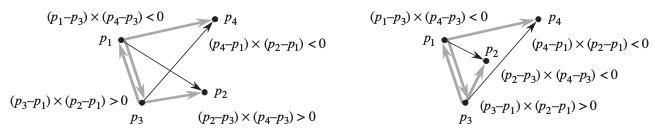
\includegraphics[scale=0.7]{line_intersect}
\end{figure}


There's an edge case: if the linge segment intersect at endpoints
then some of the cross products will be zero, so we have to check
for that. Runtime is constant. 


\subsubsection{Segment Pair intersection/Bentley-Ottmann}

Given a set of line segments $S$ figure out whether any pair intersect.
The naive algorithm is obviously $O\left(n^{2}\right)$. The faster
algorithm takes $O\left(n\lg n\right)$ and uses a ``sweep line'':
a data structure the keeps track lines intersected as an imaginary
line is ``swept'' across the set of lines. 

To line segments $s_{1},s_{2}$ are \textbf{comparable} at coordinate
$x$ if the vertical sweep line with $x$-coordinate $x$ intersects
both of them. $s_{1}$ is \textbf{above} $s_{2}$ if $s_{1},s_{2}$
are comparable and the intersection of $s_{1}$ with the sweep line
is above the intersection of $s_{2}$ with the sweep line. Being above
is a total preorder: the relation is transitive and if $s_{1},s_{2}$
are comparble at $x$ then either $s_{1}$ is above $s_{2}$, or $s_{2}$
is above $s_{1}$, or both (if $s_{1},s_{2}$ intersect at the sweep
line with $x$-coordinate $x$).

The sweep lines algorithm manages two sets of data: \textbf{sweep-line
status}, which gives the relationships between objects the sweep line
intersects, and \textbf{event-point} \textbf{schedule}, which are
the $x$-coordinates of the discrete steps of sweep line. We assume
that the sweep-line status is a data structure that supports inserting
a line segment $s$, deleting a line segment $s$, inspecting any
line segments above $s$, and any line segments below $s$. We implement
all of this with cost $O\left(\lg n\right)$ using a balanced binary
search tree keyed on a sort of the line segments using comparison
by cross product. 

Assume that no three segments intersect at the same point. The key
insight of the algorithm is that two line segments that intersect
must be \emph{consecutive} in the sweep-line status at some point
in the event-point schedule. Consider the following picture 

\begin{figure}[H]
\noindent \centering{}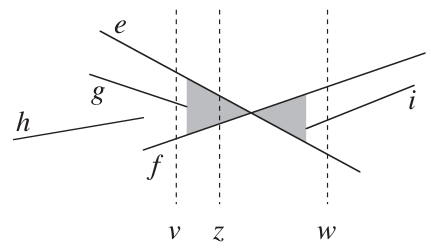
\includegraphics[scale=0.5]{third_segment}
\end{figure}


Line segments $e,f$ intersect but they are not consecutive in the
sweep-line status until after the end of line segment $g$. Supposing
$g$ were absent they would become consecutive at the beginning of
$f$. So we only need to check at left endpoints whether a line segment
intersects with line segments either below and above, or we need to
check when removing line segments whether those above and below intersect.
Here is the code. Running time is $O\left(n\lg n\right)$.

\begin{algorithm}[H]
\noindent \begin{raggedright}
\texttt{Set-Segments-Intersect}$\left(S\right)$
\par\end{raggedright}

\begin{lstlisting}[basicstyle={\ttfamily},language=Python,mathescape=true,numbers=left,showstringspaces=false,tabsize=3]
# $T$ is a binary balanced search tree with comparison being done
# by relative orientation using cross product
# so that we can fetch line segments by either left
# endpoint or right endpoint
$ left = \left\{ s\left[1\right]:s \text{ for } s\in S\right\}$
$ right = \left\{ s\left[2\right]:s \text{ for } s\in S\right\}$
$T = \text{tree}\left(\right)$
# lexicographically sort all of the endpoints in $S$
# except left endpoints should precede right endpoints
$sched = \text{sorted}\left(\left[ p\text{ for }line \in S\text{ for }p \in line \right] )\right)$
for $p \in sched$:
	if $p \in left$:
		if $p \in right$:
			return True
		else:
			$ s = left\left[p\right]$
			$\text{Insert}\left(T,s\right)$
			if $\text{Segment-Intersect}\left(\text{Above}\left(T,s\right),s\right)$ or $\text{Segment-Intersect}\left(\text{Below}\left(T,s\right),s\right)$:
				return True
	else: # $p$ is a right endpoint.
		$ s = right\left[p\right]$
		# this is the case alluded to above: if a third line segment
		# intervenes between two other line
		if $\text{Segment-Intersect}\left(\text{Above}\left(T,s\right),\text{Below}\left(T,s\right)\right)$:
			return True
		$\text{Delete}\left(T,s\right)$
return False
\end{lstlisting}
\end{algorithm}


Note that the algorithm does not find all intersections (only an intersection).
The algorithm that prints \emph{all} of the intersection is called
Bentley-Ottman and operates similarly. Instead of simply a sorted
list of event points it uses a priority queue of event points. It
then does one of 3 things depending on the type of event point
\begin{enumerate}
\item If $p$ is a left endpoint of a line segment $s$, then insert $s$
into the $T$, and if $s$ intersects a neighbor then insert their
intersection point to the priority queue (computing the intersection
point can be done in constant time by solving the system of equations
defining the two lines that correspond to the line segments).
\item If $p$ is right endpoint, then check the intersection of its neighbors,
and delete $p$ from $T$. If the neighbors intersect then add their
intersection point to the priority queue.
\item If $p$ is an intersection point of two lines segments $s_{1},s_{2}$,
then print, and exchange their order in $T$. If the new neigbhors
of $s_{1},s_{2}$ intersect with either $s_{1}$ or $s_{2}$ then
insert those intersection points.
\end{enumerate}
Running time for $k$ intersections is $O\left(\left(n+k\right)\lg n\right)$.


\subsubsection{Convex hull - Graham's Scan}

Graham's scan solves the problem of finding the convex hull by maintaining
a stack of candidate points while traversing a list of all of the
points sorted by polar angle in counter-clockwise order. For each
new point it figures out whether the new point constitutes a left
turn or right turn relative to the existing candidate points. If the
point makes a right turn then the point it pivots around isn't in
the convex hull, so that point should be removed, and so on until
the new point being considered makes a left turn. This picture should
illustrate the process

\begin{figure}[H]
\noindent \centering{}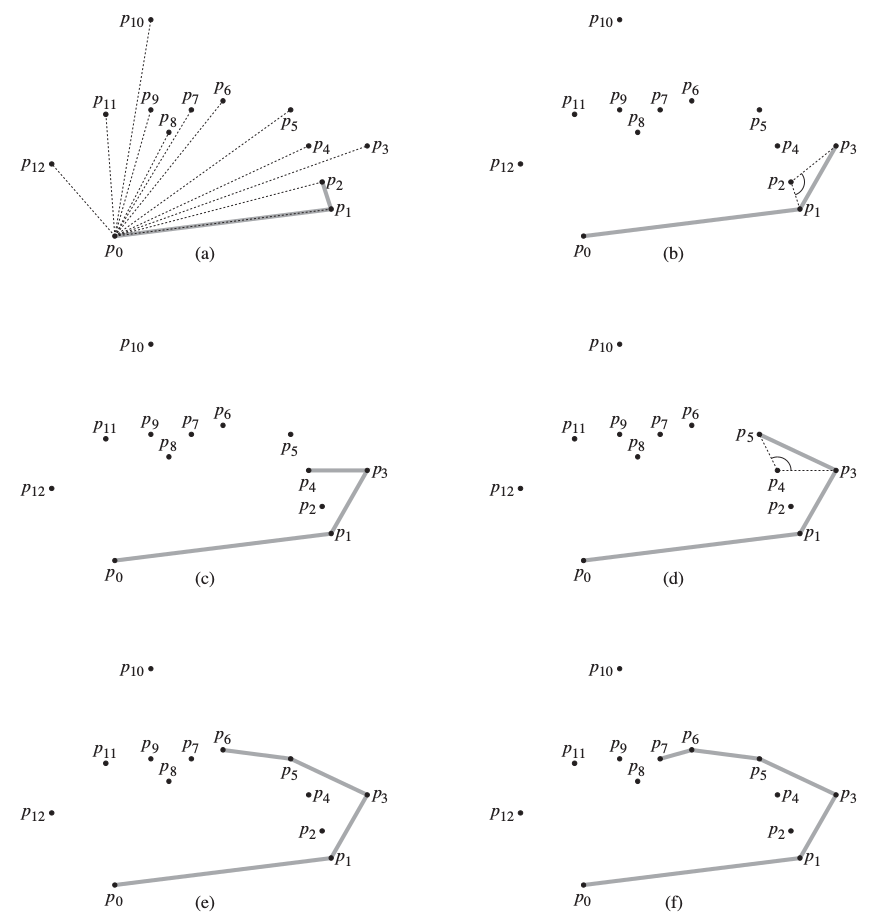
\includegraphics[scale=0.4]{grahams}
\end{figure}


The running time is $O\left(n\lg n\right)$.


\subsubsection{Jarvis March}

Jarvis march is another convex hull finding algorithm that ``gift
wraps'' the set of points: starting with the most south-eastern point
it searchs out the point with the shallowest counter-clockwise angle
i.e. ``rightest'' turn (which is the next point in the convex hull).
Running time is $O\left(nh\right)$ where $h$ is the number of points
in the convex hull.


\subsubsection{Closest pair of points}

Given a set of points $Q=\left(\left[x_{1},\dots,x_{n}\right],\left[y_{1},\dots,y_{n}\right]\right)$
find the pair of points $p_{i},p_{j}=\left(x_{i},y_{i}\right),\left(x_{j},y_{j}\right)$
that minimize $\left\Vert p_{i}-p_{j}\right\Vert $. The naive algorithm
(try all pairs) obviously runs in $O\left(n^{2}\right)$. The following
divide and conquer algorithm runs faster.

Each recursive call takes a subset $P\subset Q$ and arrays $X,Y$
of presorted points; $X$ is sorted in monotonically increasing $x$-coordinate
and $Y$ in monotonically increasing $y$-coordinate. 

If $\left|P\right|\leq3$ then just brute force it. Otherwise
\begin{itemize}
\item \textbf{Divide}: split the points according to $x$-coordinate into
two sets $P_{L}=\left\lceil \left|P\right|/2\right\rceil $ and $P_{R}=\left\lfloor \left|P\right|/2\right\rfloor $.
More on how to compute the corresponding $X_{L},Y_{L}$ and $X_{R},Y_{R}$
in the code.
\item \textbf{Conquer}: Recurse into $P_{L},X_{L},Y_{L}$ and $P_{R},X_{R},Y_{R}$
computing $\delta_{L}$ and $\delta_{R}$ (the minimum distances in
the recursions).
\item \textbf{Combine}: the closest pair with is either $\delta=\min\left\{ \delta_{L},\delta_{R}\right\} $
or a pair points with one in $P_{L}$ and one in $P_{R}$. Note that
for a pair of points to be closer than $\delta$ they must each be
with $\delta$ of the line that was used to create the partition $P_{L},P_{R}$.
The following picture shows the intuition


\begin{figure}[H]
\noindent \centering{}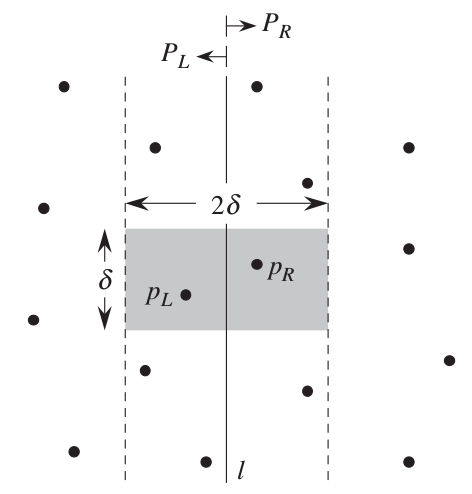
\includegraphics[scale=0.3]{2d}
\end{figure}



To find these points
\begin{enumerate}
\item Construct the array $Y'$ with only the points with $x$-coordinate
within $\delta$ of the line separating $P_{L},P_{R}$. Maintain the
order of $Y$.
\item For each point $p\in Y'$, consider only the following (in the order)
7 points. This is sufficient because at most $7$ points can fit in
the $2\delta\times\delta$ patch around any $p\in Y'$; consider the
picture


\begin{figure}[H]
\noindent \centering{}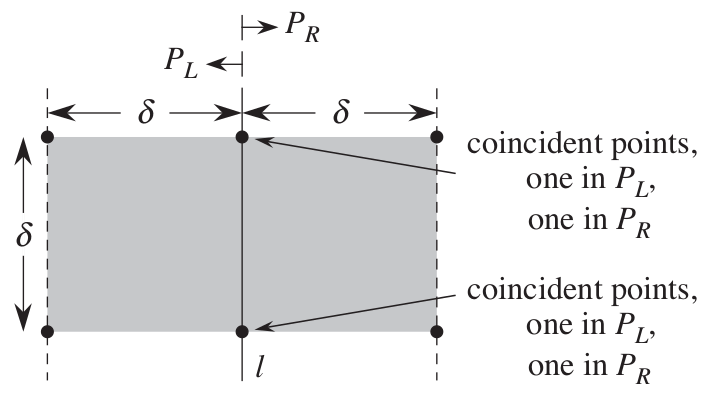
\includegraphics[scale=0.3]{8points}
\end{figure}


\end{enumerate}
\end{itemize}
The total running time is $O\left(n\lg n\right)$.
\end{document}
